\documentclass[12pt,a4j]{jarticle}
\floatsep=10mm
\textfloatsep=10mm
\usepackage[dvips]{graphicx}
\usepackage{graphicx}
\usepackage{amscd}
\usepackage{multirow}
\usepackage{epsfig}
\usepackage{amsmath,amssymb,epsf}
\usepackage{comment}
\usepackage{graphicx,psfrag}
\usepackage{bm}
\def\vec#1{\mbox{\boldmath$#1$}}
\def\sgn#1{\mbox{sgn($#1$)}}
\def\c#1{^{#1}}
\def\argmin#1{\underset{#1}{\mbox{argmin}}}
\def\leqq{\le}
\def\geqq{\ge}
%%%$B%Z!<%8%l%$%"%&%H$N%W%j%"%s%V%k(B%%%%
\setlength{\unitlength}{1mm}
\setlength{\topmargin}{-1cm}
\setlength{\oddsidemargin}{-0.55cm}
\setlength{\evensidemargin}{-0.55cm}
\setlength{\textheight}{24cm}
\setlength{\textwidth}{17cm}
\renewcommand{\baselinestretch}{1.3}

%%%%%%%%%%%%%$B?^I=$N3d9g(B%%%%%%%%%%%%%%%
\setcounter{topnumber}{5}%    $B%Z!<%8>eIt$N?^I=$O(B 5 $B8D$^$G(B
\def\topfraction{1.00}%       $B%Z!<%8$N>e(B 1.00 $B$^$G?^I=$G@j$a$F2D(B
\setcounter{bottomnumber}{5}% $B%Z!<%82<It$N?^I=$O(B 5 $B8D$^$G(B
\def\bottomfraction{1.00}%    $B%Z!<%8$N2<(B 1.00 $B$^$G?^I=$G@j$a$F2D(B
\setcounter{totalnumber}{10}% $B%Z!<%8$"$?$j$N?^I=$O(B 10 $B8D$^$G(B
\def\textfraction{0.1}%      $B%Z!<%8$&$AK\J8$,@j$a$k3d9g$N2<8B(B
\def\floatpagefraction{0.6}%  $B?^I=$@$1$N%Z!<%8$O>/$J$/$H$b$3$l$@$1$r?^I=$,@j$a$k(B


%\documentclass[12pt,a4j,epsf,amstex,righttag]{jarticle}
%%%%%%%%%%%% $B0J2<$O(BLinux $B$N(B Latex2e $B$G%3%s%Q%$%k$9$k$H$-(B
% rcp hirata.tex izanagi:~/tex/sotu/sotu98/
%%%%%%%%%%%% (mule$B$G$N%-!<A`:n$O(B^ctj)

%%%%%%%%%%%%% $B0J2<$O(BUnix $B$N(B amslatex $B$G%3%s%Q%$%k$9$k$H$-(B
%\documentstyle[12pt,a4j,epsf,amstex,righttag]{jarticle}
%\def\myepsfile#1#2#3{\epsfile{file=#1,width=#2}}
%%%%%%%%%%%%% $B0J>e$O(BUnix $B$N(B amslatex $B$G%3%s%Q%$%k$9$k$H$-(B

% $B%0%i%U%#%C%/%9$N;HMQ(B
%\usepackage[dvips]{graphicx}
% -- AMS$B%Q%C%1!<%8!&(BAMSFonts
%\usepackage{amsmath,amssymb}
% $B?t<0MQ%U%)%s%H(B
%\\usepackage{mathptmx}
%\setlength{\topmargin}{.5cm}
%\setlength{\unitlength}{1mm}
\def\dint_#1^#2{\displaystyle{\int_{#1}^{#2}}}
\def\tint_#1^#2{\textstyle{\int_{#1}^{#2}}}
\def\dfrac#1#2{\displaystyle{\frac{#1}{#2}}}
\def\tfrac#1#2{\textstyle{\frac{#1}{#2}}}
\def\textem#1{\textit#1}
\def\vec#1{\mbox{\boldmath$#1$}}
\def\argmin#1{\underset{#1}{\mbox{argmin~}}}
\def\argmax#1{\underset{#1}{\mbox{argmax~}}}
\def\RealNumSet{\Bbb R}
%\def\exp#1{e^{#1}}
%\def\eqn#1{(\ref{#1})}
%\def\refeq#1{$B<0(B(\ref{#1})}
%\def\reffig#1{$B?^(B\ref{#1}}
%\def\reftab#1{$BI=(B\ref{#1}}
%\def\aratio{\theta_{\alpha}}
%\def\eratio{\theta_{H}}
%\def\reinitratio{\theta_{r}}
%\renewcommand{\floatpagefraction}{1}
%\renewcommand{\topfraction}{1}
%\renewcommand{\bottomfraction}{1}
%\renewcommand{\textfraction}{0}
%\renewcommand{\theequation}{\thesubsection.\arabic{equation}}
\def\bg{{\bf{bg}}}
\def\ob{{\bf{ob}}}
\def\ib{{\bf{ib}}}
\def\tst{{\bf{tst}}}
\def\bst{{\bf{bst}}}
\def\tr{{\bf{tr}}}
\def\bs{{\bf{bs}}}
\def\bb{{\bf{bb}}}
\def\mse{{\bf{MSE}}}
\def\mae{{\bf{MAE}}}
\def\mxae{{\bf{MxAE}}}

\begin{document}

\title{\vspace{4cm}  
$BB46HO@J8(B\\
\vspace{1cm}
$BCO<'5$J}0L%;%s%5$HCO?^>pJs$rMQ$$$k%Q!<%F%#%/%k%U%#%k%?(B
$B$K$h$k20300\F0%m%\%C%H$N<+8J;Q@*?dDj7k2L$N=$@5(B
\vspace{4cm}  
}

\author{$B;XF36541!'9uLZ(B $B=(0l(B $B65<x(B\\
$B6e=#9)6HBg3X(B  $B9)3XIt(B\\
$B5!3#CNG=9)3X2J(B  $BCNG=@)8f9)3X%3!<%9(B\\
$B3X@RHV9f(B $B!'(B 14104018\\
$BDs=P<T;aL>(B $B!'1sF#!!8w(B}
\date{$BDs=PF|(B $B!'(B 2018$BG/(B2$B7n(B14$BF|(B}

%%%% $BI=;f(B  %%%%%
\titlepage
\maketitle
\thispagestyle{empty}
\newpage

%%%% $BE&MW(B %%%%%
\begin{center}{\Large $BE&MW(B}\end{center}
 $B!!K\8&5f$G$O(B, $B0\F0%m%\%C%H$,2030$G3hF0$7$?8e(B, $BF@$i$l$?(B
$B<+8J;Q@*?dDj7k2L$r(B, $BJ#?t$N%;%s%5>pJs$rMQ$$$F=$@5$r9T$C$?(B. $B0\F0(B
$B%m%\%C%H$K$O(BMobileRobots$B<R$N(BPioneerP3-AT$B$r;HMQ$7(B, Kinect$B%;%s%5$K$h$jF@$i$l$k(B3$B<!(B
$B85(BSLAM$B$N<+8J;Q@*?dDj7k2L$r(B, $BCO<'5$J}0L%;(B
$B%s%5$N>pJs$HCO?^>pJs$rMQ$$$k%Q!<%F%#%/%k%U%#%k%?$K$h$j(B, $B=$@5$r9T$&$H$$$&(B
$B<jK!$r;n$_$?(B. 

 $B$3$l$^$G(B, $B2f!9$N8&5f<<$G$O(B, $B%*%I%a%H%j>pJs$h$j%@%$%J%_%/%9(B
$B$r9=@.$7(B, GPS$B$HCO<'5$J}0L%;%s%5$*$h$S(BKinect$B%;%s%5$rMQ$$$k%Q!<%F%#%/%k(B
$B%U%#%k%?$K$h$k<+8J;Q@*?dDj$r9T$C$?(B. $B$=$N7k2L(B, Kinect$B%;%s%5$h$j(B, $B@:EY$N9b$$<+8J;Q@*?d(B
$BDj7k2L$rF@$?(B. $B$7$+$7(B, GPS$B$NB,Dj8m:9$,Bg$-$$$3$H$d(B, Kinect$B%;%s%5$rMQ$$$F(B
$BF@$i$l$?(B3$B<!85%G!<%?$N9b$5>pJs$rL5;k$7$FL`EY7W;;$r9T$&$H$$$&LdBj$,$"$C$?(B. $B$=$3$G(B, $BK\8&5f(B
$B$N<jK!$K<h$jAH$_(B, $B$=$N7k2L(B, $B@:EY$N9b$$(B, $B<+8J;Q@*?dDj7k2L$N=$@5$r9T$&$3$H$,(B
$B$G$-$?(B.
\thispagestyle{empty}
\newpage
\setcounter{page}{1}

%%%% $BL\<!(B %%%%%
\tableofcontents
\newpage


%%%%%%% $BK\J8(B %%%%%%%% 
\section{$B=xO@(B}
   $B%m%\%C%H$,2030$G3hF0$9$k$?$a$K$O(B, $B@53N$J<+8J;Q@*?dDj$,I,MW$G$"$k(B. $B2f!9$N(B
$B8&5f<<$G$O$3$l$^$G(B, $B%*%I%a%H%j>pJs$h$j%@%$%J%_%/%9(B
$B$r9=@.$7(B, GPS$B$HCO<'5$J}0L%;%s%5$*$h$S(BKinect$B%;%s%5$rMQ$$$k%Q!<%F%#%/%k(B
$B%U%#%k%?$K$h$k<+8J;Q@*?dDj$r9T$C$?(B. $B$=$N7k2L(B, Kinect$B%;%s%5$h$j(B, $B@:EY$N9b$$<+8J;Q@*?d(B
$BDj7k2L$rF@$?(B. $B$7$+$7(B, GPS$B$NB,Dj8m:9$,Bg$-$$$3$H$d(B, Kinect$B%;%s%5$rMQ$$$F(B
$BF@$i$l$?(B3$B<!85%G!<%?$N9b$5>pJs$rL5;k$7$FL`EY7W;;$r9T$&$H$$$&LdBj$,$"$C$?(B. 

  $B$=$3$G(B, $BK\8&5f$G$O(B, Kinect$B%;%s%5$K$h$jF@$i$l$k(B3$B<!85(BSLAM$B$N<+8J;Q@*?dDj7k2L$r(B, $BCO<'5$J}0L%;(B
$B%s%5$N>pJs$HCO?^>pJs$rMQ$$$k%Q!<%F%#%/%k%U%#%k%?$K$h$j(B, $B=$@5$r9T$&$H$$$&(B
$B<jK!$r;n$_$?(B. $BK\9F$G$O!$(B2$B>O$G<+8J;Q@*?dDj7k2L$r=$@5$9$k<jK!$r<($7(B, 3$B>O$G<B837k2L$r<($9$H$H$b$K9M;!$r9T$$!$(B4$B>O$G7kO@$r=R$Y$k!%
\newpage


\section{$BCO<'5$J}0L%;%s%5$HCO?^>pJs$rMQ$$$k%Q!<%F%#%/%k%U%#%k%?(B(PF)$B$K$h$k<+8J;Q@*?dDj$N=$@5(B}
 \subsection{$BCO?^>pJs$rMQ$$$k(BPF$B$K$h$k<+8J;Q@*?dDj(B}
  \subsubsection{$BCO?^>pJs$N:n@.(B}
  $BK\8&5f$GMQ$$$kCO?^>pJs$O%0!<%0%k%^%C%W$rMQ$$$F:n@.$9$k!%%0!<%0%k%^%C%W$h$j(B, $B<B:]$KAv9T$7$?F;O)(B
$B$NCf1{IU6a$NJ#?tE@$N0^EY(B, $B7PEY$r<hF@$7(B, $BKL$r(B$y$$B<4J}8~(B, $BEl$r(B$x$$B<4J}8~$H$7(B
$B$?@$3&:BI8$X$HJQ49$9$k(B. $B;~9o(B$k$$B$G$NKL0^!$(B
$BEl7P$r(B$N_{k}$$B!$(B$E_{k}$$B$H$9$k$H!$El7P$NJQ49$O(B
\begin{equation}
 x_{k}
  =(E_{k}-E_{0})
  \frac{\beta}{360}\
  cos\left(\frac{\pi N_{0}}{180}\right)
\end{equation}
$B$H$J$k!%$3$3$G(B$\beta$$B$O@VF;D9$G(B$40075.017$[km]$B$G$"$k!%F1;~$KKL0^$O(B
\begin{equation}
 y_{k}=(N_{k}-N_{0})\frac{\pi\gamma}{360}
\end{equation}
$B$H$J$k!%$3$3$G(B$\gamma$$B$OKL6K$HFn6K$r7k$s$@D>7B$G(B$12756.274$[km]$B$G$"$k!%(B


$B<hF@$7$?E@(B$\vec{m}_{i}=({x_i},{y_i})(i=1,2,3,4,5)$$B$r7k$S(B,
$BCO?^>pJs(B${\it{R}}=\{\vec{x} \mid
\vec{x}=\alpha(\vec{m}_{j+1}-\vec{m}_{j})+\vec{m}_{j}\}(0<\alpha\leq 1,
j=1,2,3,4 , \vec{m}_{5}=\vec{m}_{1})$
$B$H$7$F;HMQ$9$k!%:n@.$7$?7PO)>pJs$r%0!<%0%k%^%C%W$KI=<($7$??^$r?^(B\ref{$BCO?^>pJs(B}$B$K<($9!%(B

\begin{figure}[h]
 \begin{center}
  \begin{tabular}{cc}
   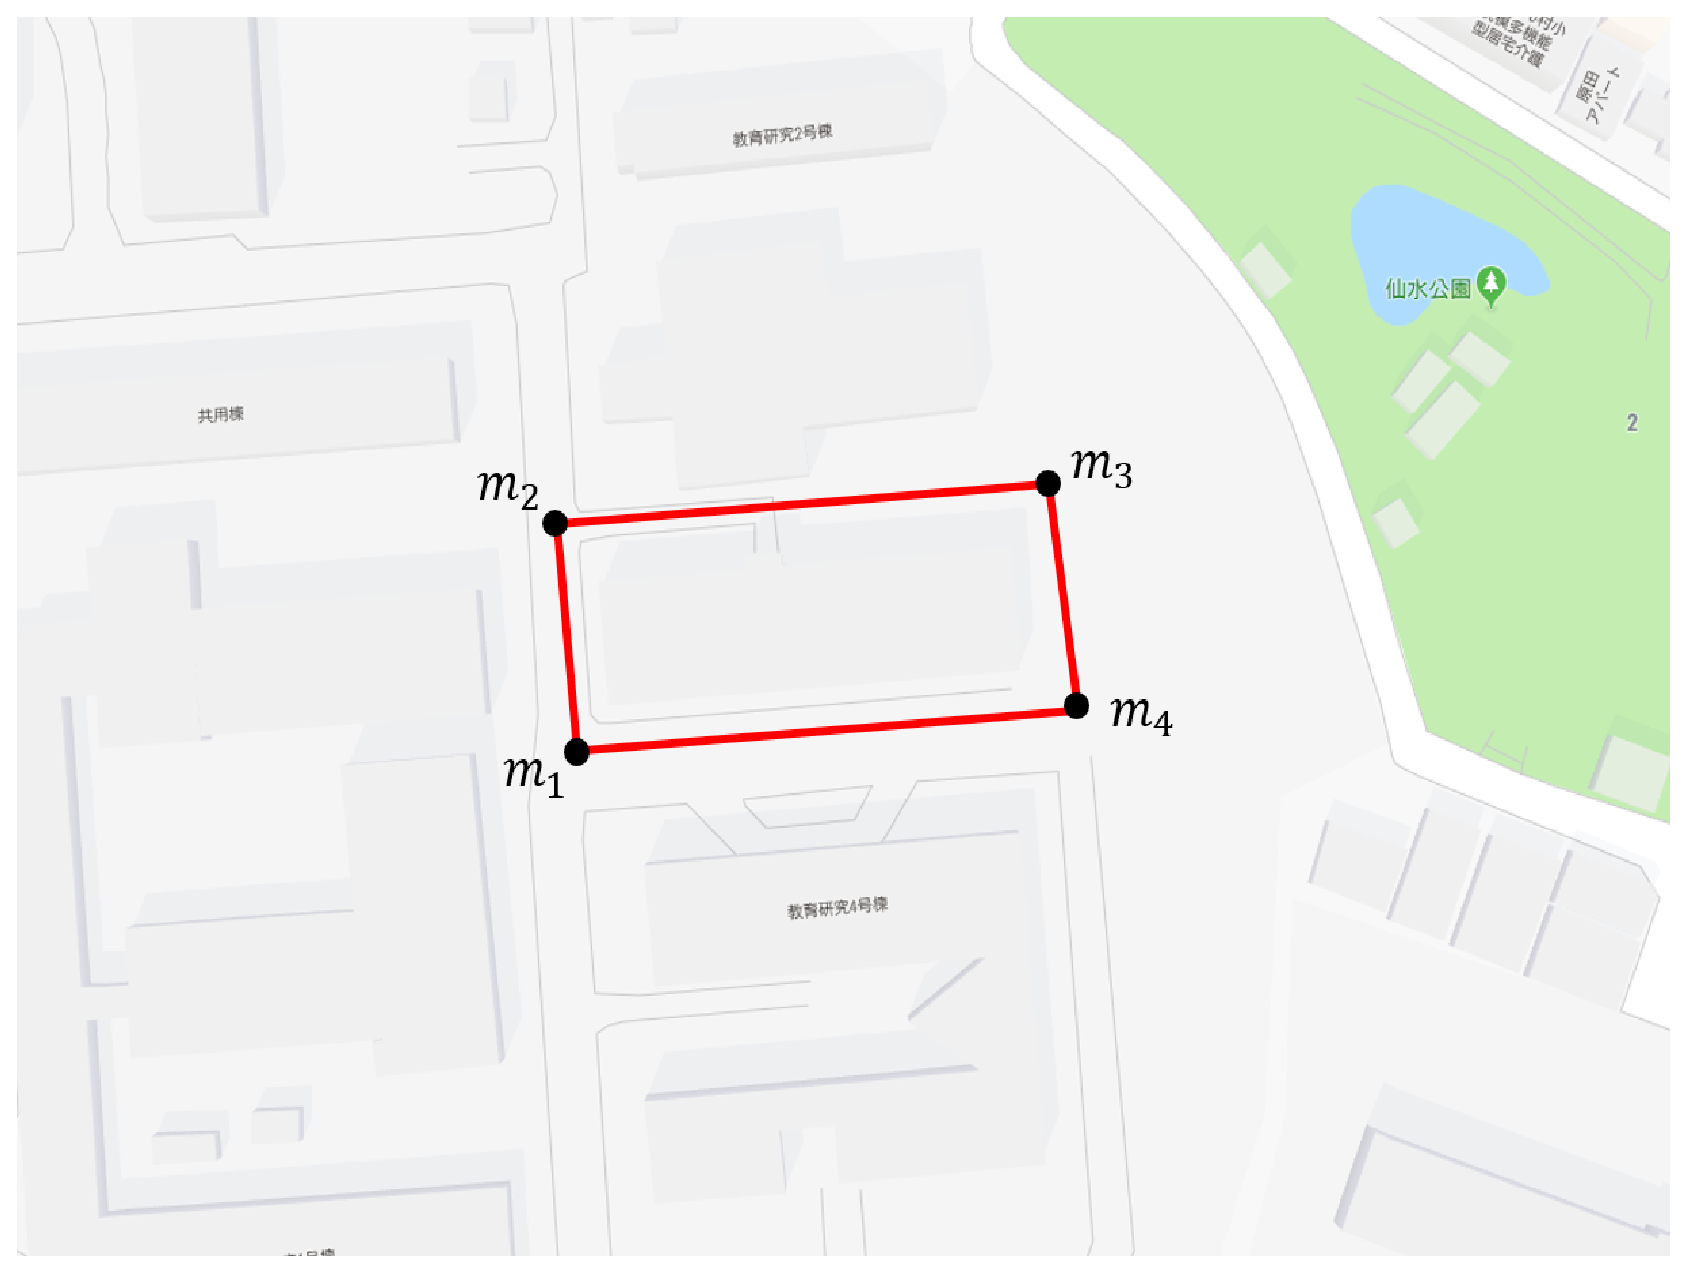
\includegraphics [height=5.0cm,width=8.0cm] {./fig/gpst.eps}
  \end{tabular}
 \end{center}
 \caption{$BCO?^>pJs(B}\label{$BCO?^>pJs(B}
\end{figure}
\clearpage
\newpage
  \subsubsection{$BJ}0L%;%s%5$N?.MjEY(B}
  $B@h9T8&5f$G$O(BGPS$B$HCO<'5$J}0L%;%s%5$*$h$S(BKinect$B%;%s%5$rMQ$$$k(BPF$B$K$h$j<+8J(B
$B;Q@*?dDj$r9T$$(B, Kinect$B%;%s%5$h$jNI$$7k2L$,F@$i$l$k$3$H$,J,$+$C$?(B. $BK\8&5f(B
$B$G$O(B, Kinect$B%;%s%5$N%G!<%?$+$iF@$i$l$?<+8J;Q@*?dDj7k2L$rCO?^>pJs$HCO<'5$(B
$BJ}0L%;%s%5$rMQ$$$F=$@5$9$k$3$H$rL\E*$H$9$k(B. $BCO<'5$J}0L%;%s%5$K$h$jF@$i$l(B
$B$?%G!<%?$r?^(B\ref{deg}$B$K<($9(B. $B$3$N?^$+$i0lDj;~4V$*$-$K%m%\%C%H$,$*$h$=(B90
$BEY$:$D2sE>$7$F$*$j(B, $B%m%\%C%H$,<B:]$K0\F0$7$?7PO)$K1h$C$?%G!<%?$r<hF@$7$F(B
$B$$$k$3$H$,$o$+$k(B.



\begin{figure}[h]
 \begin{center}
  \begin{tabular}{cc}
   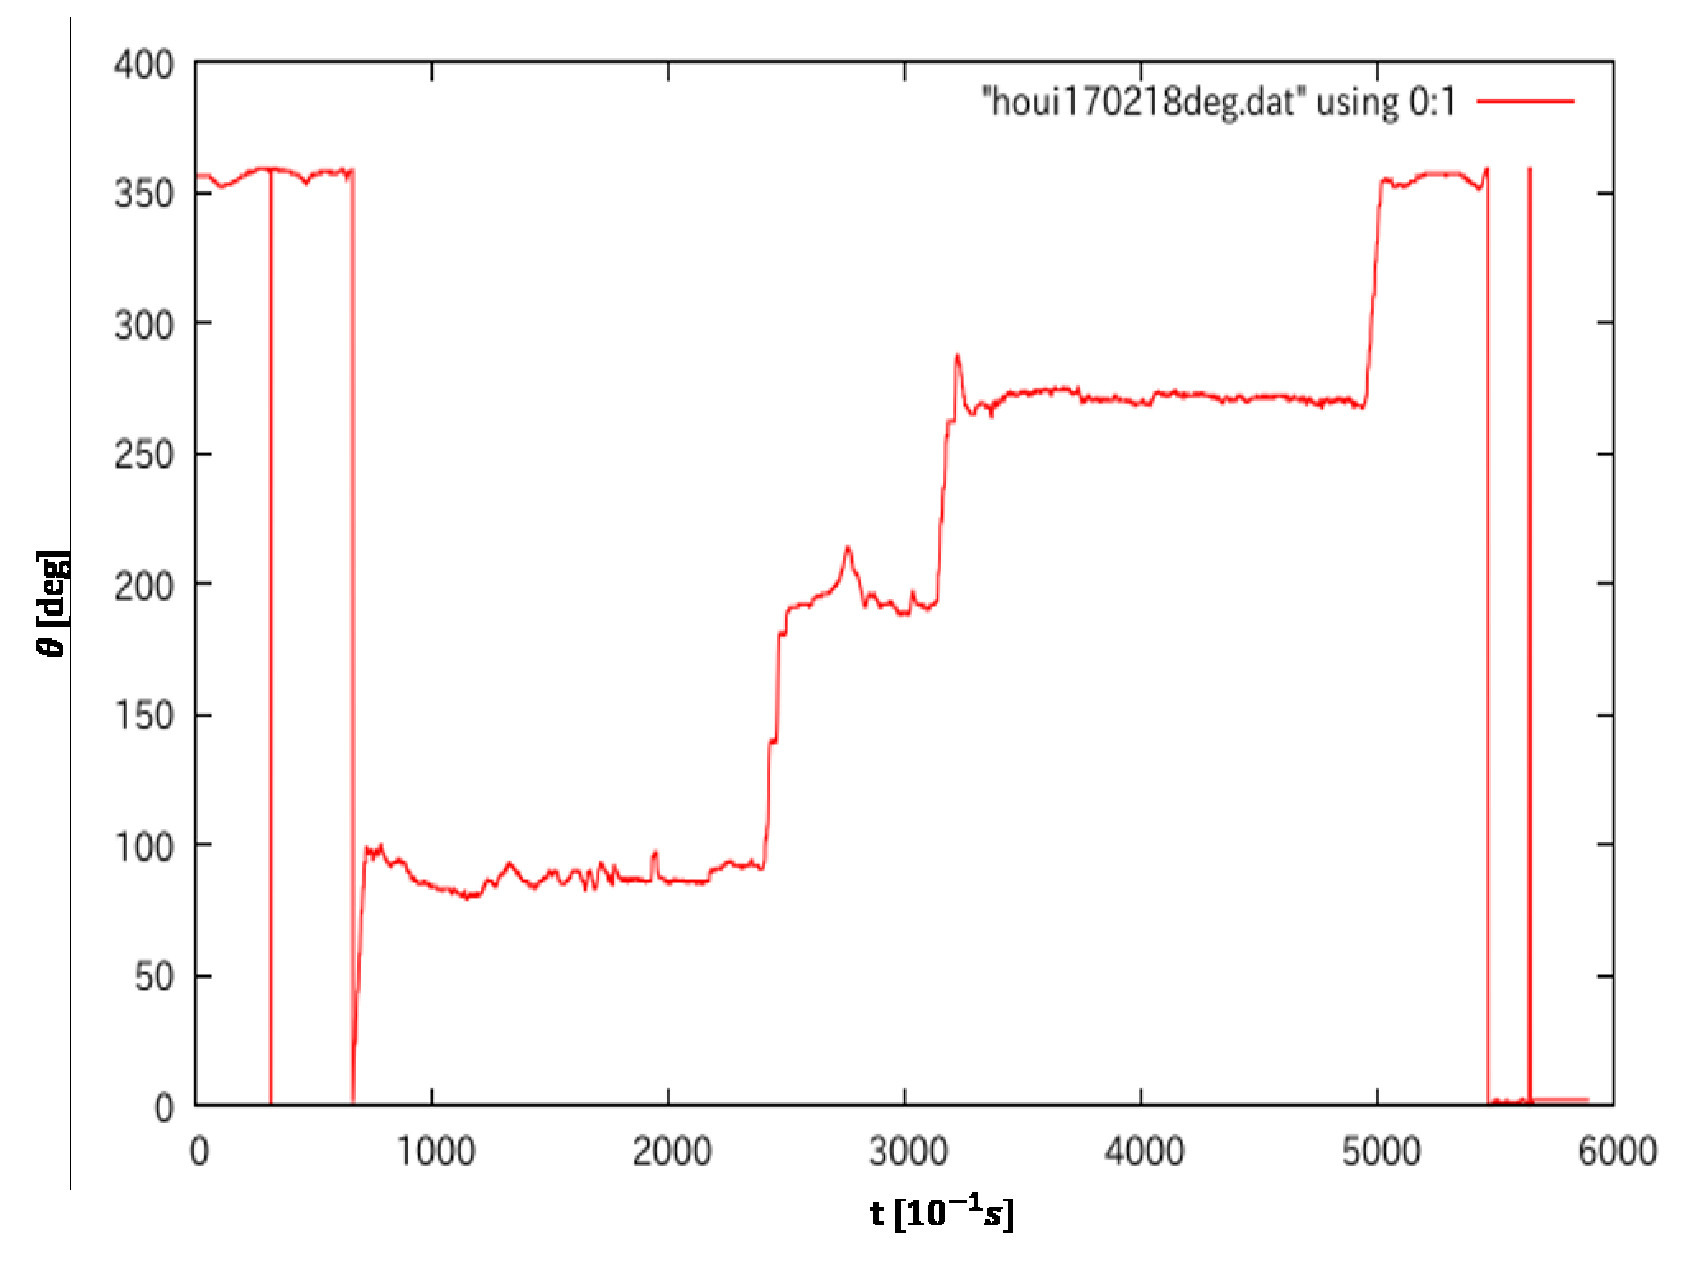
\includegraphics [height=8cm,width=11cm] {./fig/houiend.eps}
   \end{tabular}
  \end{center}
 \caption{$BCO<'5$J}0L%;%s%5$N%G!<%?(B}\label{deg}
\end{figure}
\newpage
  \subsubsection{PF$B$K$h$k<+8J;Q@*?dDj%"%k%4%j%:%`(B}
  $B%Q!<%F%#%/%k%U%#%k%?(B(PF)$B$H$O3NN(L)EYJ,I[$rB??t$N%5%s%W%k$K$h$C$F6a;w$9$k<jK!$N0l$D$G$"$k!%>uBV6u4VCf$N%Q!<%F%#%/%k$H8F$P$l$kB??t$NN3;R$K$h$j!$%m%\%C%H$N;Q@*$K4X$9$k2>@b$rJ#(B
$B?tN)$F$k$3$H$K$h$jJ,I[$r6a;w$7!$$=$l$rDI@W!$;~4V99?7$9$k%"%k%4%j%:%`$G$"(B
$B$k!%K\8&5f$G<BAu$9$k(BPF$B$N%"%k%4%j%:%`$r0J2<$K4J7i$K<($9!%>0!$K\8&5f$K9g$o(B
$B$;$F2f!9$N8&5f(B
$B<<$G=>Mh$N<+8J;Q@*?dDj$KMQ$$$i$l$F$$$?$b$N$r2~NI$7$F$*$j!$@h9T8&5fO@J8$G$b(B
$B>R2p$5$l$F$$$k$b$N$r0lIt;29M$K$7$F$$$k!%(B[1]\\
 $B$^$:!$;~9o(B$k$$B$G$N%m%\%C%H$N;Q@*$r(B
 $\vec{x}_{k}=(x_{k},y_{k},z_{k},\theta_{k})^T$$B$H$7!$$=$N;~9o$N;Q@*$K(B
 $B$D$$$F$N3F%Q!<%F%#%/%k$NJ,I[$r(B$r(\vec{x}_{k})$$B$H$9$k!%$3$N$H$-!$%Q!<%F%#%/%k72(B
$\bigl< \vec{X}_{k}^{[m]} \bigr>_{m=1}^{M}$$B$K$h$k6a;w$O(B
$\bigl< \vec{X}_{k}^{[m]} \bigr>_{m=1}^{M}
=\bigl<\vec{x}_{k}^{[m]},w_{k}^{[m]} \bigr>_{m=1}^{M}$
$B$N$h$&$KM?$($i$l$F$$$k$b$N$H$9$k!%$3$3$G!$(B$M$$B$O%Q!<%F%#%/%k?t$G$"$j!$3F!9(B
$B$N;Q@*(B$\vec{x}_{k}^{[m]}$$B$H$=$N=E$_(B($BL`EY(B)$w_{k}^{[m]}$$B$r$b$DJ#?t$N%Q!<(B
$B%F%#%/%k$K$h$j!$%Q!<%F%#%/%k72$,9=@.$5$l$k!%$3$3$G>eE:;z(B$[m](m=1,2,\cdots,M)$
$B$O%Q!<%F%#%/%k$N%$%s%G%C%/%9$rI=$7$F$*$j!$3F=E$_(B$w_{k}^{[m]}$$B$O(B
$0 \leq w_{k}^{[m]} \leq 1$$B!$(B$\sum_{m=1}^{[M]} w_{k}^{[m]}=1$
$B$rK~$?$9$b$N$H$9$k!%(B\par
PF$B$O0J2<$N(B$3$$B%9%F%C%W$N=hM}$r9T$&!%$?$@$7!$;~9o(B$0$$B$K$*$1$k=i4|>uBV$K$D$$$F$O(B
$B$9$Y$F$N%Q!<%F%#%/%k$KBP$7!$(B
$\bigl< \vec{X}_{0}^{[m]} \bigr>_{m=1}^{M}
=\bigl< \vec{x}_{0}^{[m]},w_{0}^{[m]} \bigr>_{m=1}^{M}
=\bigl< (0,0,0,0)^T,\frac{1}{M} \bigr>_{m=1}^{M}$
$B$HM?$($F$*$/$b$N$H$9$k!%(B
\begin{enumerate}
 \item[Step 1:]{\bf $B;Q@*?dDj(B}\par
$B%m%\%C%H$N0LCV(B$\vec{x}_{k}=({x}_{k},{y}_{k},{z}_{k})^T$$B$H;~9o(B${T}_{k}$$B$,(B
$BM?$($i$l$F$$$k$H$9$k$H(B, $\vec{x}_{k}$$B$+$i(B$\vec{x}_{k+1}$$B$K9T$/B.EY$O<!$N$h$&$K?dDj$5$l$k(B.
\begin{equation}
 \vec{v}_{k}=\frac{\vec{x}_{k+1}-\vec{x}_{k}}{{T}_{k+1}-{T}_{k}}=
\frac{\Delta \vec{x}_{k}}{\Delta {T}_{k}}
\end{equation}
$B$h$C$F(B, $B0LCV$N;~4VJQ2=$O(B
\begin{equation}
\vec{x}_{k+1}=\vec{x}_{k}+\vec{v}_{k}\Delta \vec{T}_{k}
\end{equation}
$B$H?dDj$G$-$k(B. $B$^$?(B, $\theta_{k}$$B$O?^(B\ref{sokudo2}$B$K<($7$?3QEY$H$7$?(B.
\begin{figure}[h]
 \begin{center}
  \begin{tabular}{cc}
   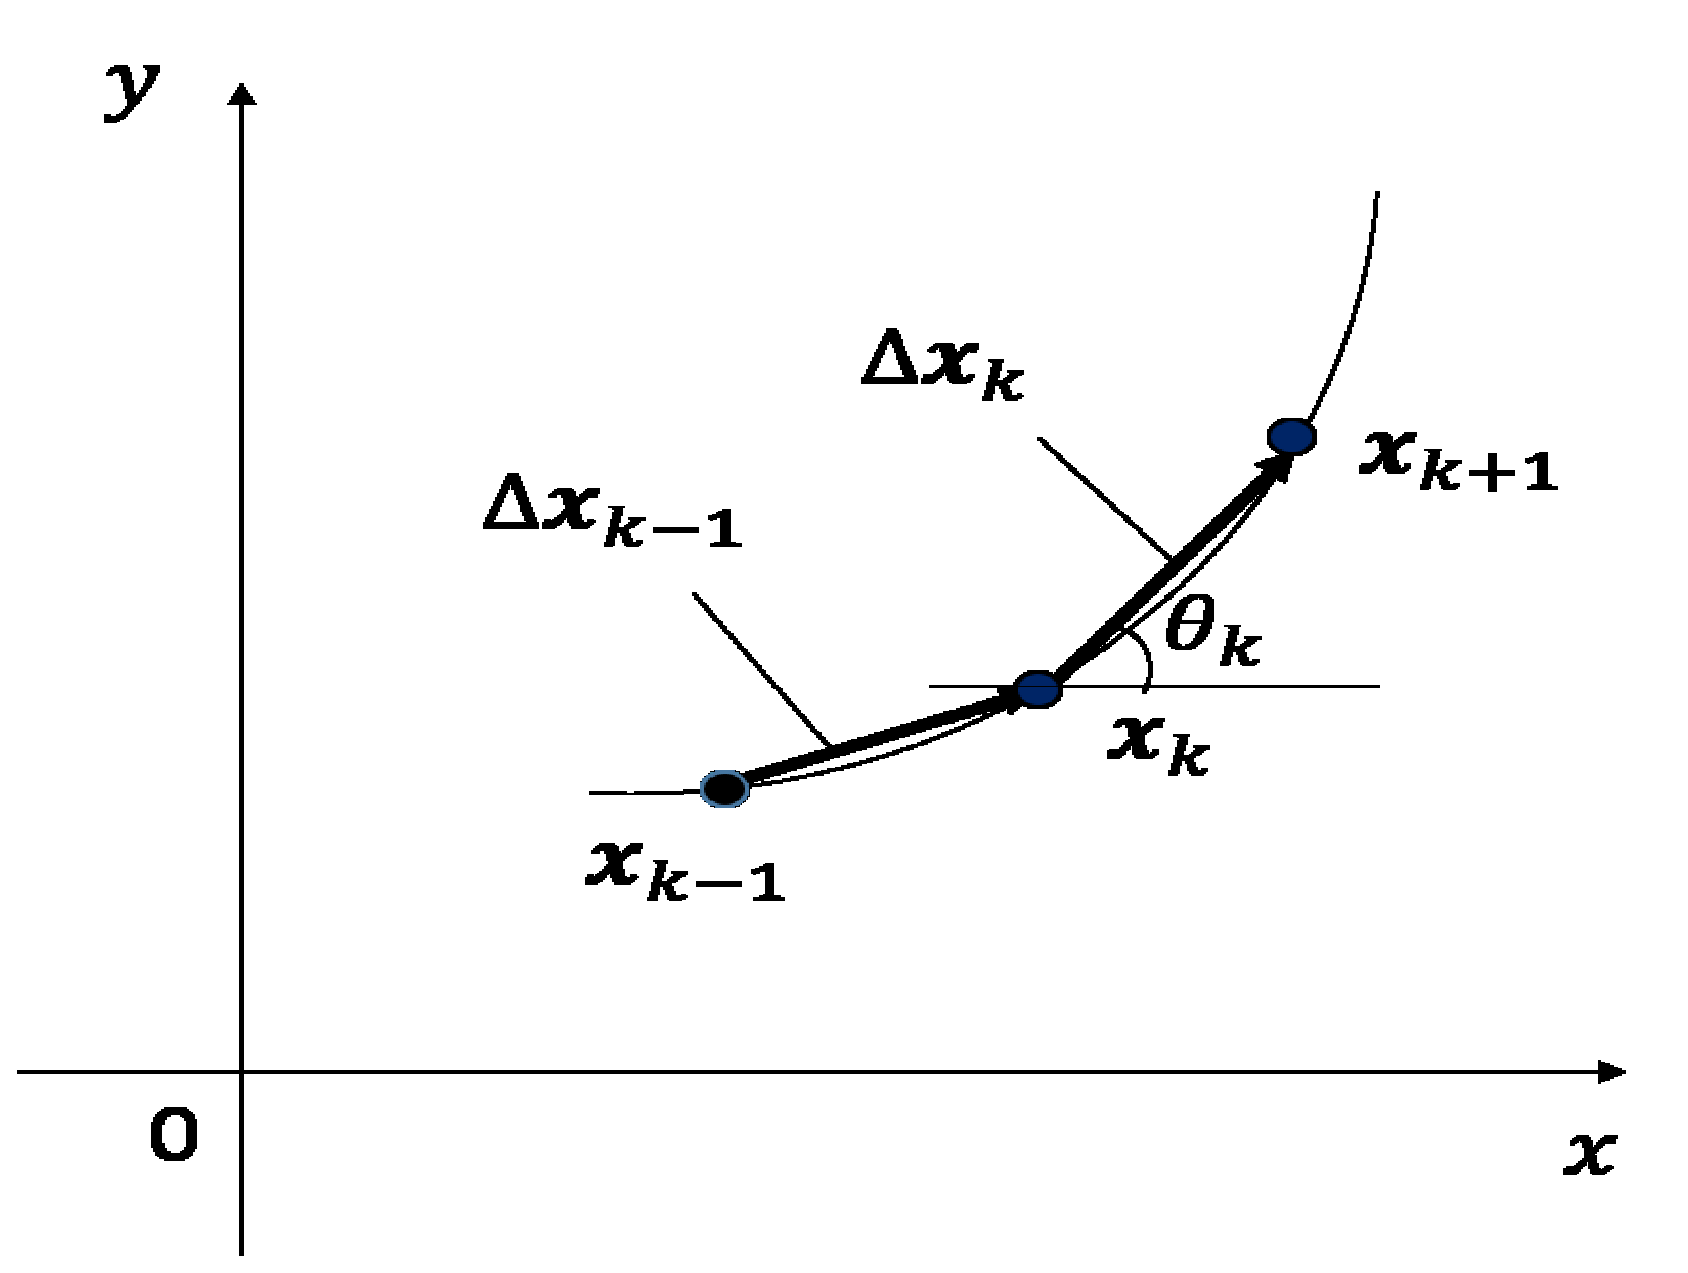
\includegraphics [height=5.0cm,width=5.0cm] {./fig/sokudo2.eps}
  \end{tabular}
 \end{center}
 \caption{$BB.EY$NF3=P(B}\label{sokudo2}
\end{figure}

\begin{comment}
$B;~9o(B$k$$B$K$*$1$k;Q@*(B$\vec{x}_{k}^{[m]}$$B$H%m%\%C%H$N@)8fF~NO(B
$\vec{u}_{k}$$B$,M?$($i$l$?2<$G!$<!;~9o(B$k+1$$B$K$*$1$k;Q@*(B$\vec{x}_{k+1}$
$B$K4X$9$kDs0FJ,I[(B$\tilde{q}(\vec{x}_{k+1})$$B$K=E$_(B$w$$B$rIU2C$7!$%Q!<%F%#%/%k72(B
$\bigl< \tilde{\vec{X}}_{k+1}^{[m]} \bigr>_{m=1}^M
=\bigl< (\tilde{\vec{x}}_{k+1}^{[m]},\tilde{w}_{k+1}^{[m]}) \bigr>_{m=1}^{M}$
$B$r@8@.$9$k!%$3$N=hM}$OK\O@J8$NIUO?(BA$B$K=R$Y$F$$$k%m%\%C%H$NB.EYF0:n%b%G%k$rMQ$$$F!$<!;~9o$KCV$1$k%m%\%C%H$N;Q@*$N2>@b$rJ#?t%5%s%W%j%s%0$9$k$b$N$G$"$k!%$D$^$j!$3F%Q!<%F%#%/%k$4$H$K%m%\%C%H$N@)8fF~NO$K0[$J$k%N%$%:$r2C$(?7$?$J@)8fF~NO(B
$\hat{\vec{u}}_{k}^{[m]}=(\hat{v}_{k}^{[m]},\hat{\omega}_{k}^{[m]})^T
=(v_{k}+\varepsilon^{[m]},\omega_{k}+\varepsilon^{[m]})^T$
$B$r@8@.$9$k$3$H$G!$(B$\hat{\omega}_{k}^{[m]} \neq 0$$B$N$H$-$N(B
$B<!;~9o$K$*$1$k;Q@*$N2>@b(B$\tilde{\vec{x}}_{k+1}^{[m]}$$B$,<!<0$N$h$&$K5a$a$i(B
$B$l$k!%(B
\begin{equation}
 \tilde{\vec{x}}_{k+1}^{[m]}=\vec{x}_{k}^{[m]}+\left(
					      \begin{array}{c}
					       -\frac{\hat{v}_{k}^{[m]}}{\hat{\omega}_{k}^{[m]}}
						\sin{\theta_{k}^{[m]}}
						+\frac{\hat{v}_{k}^{[m]}}{\hat{\omega}_{k}^{[m]}}
						\sin{(\theta_{k}^{[m]}+\hat{\omega}_{k}^{[m]}\Delta
						t_{k})}\\
					       \frac{\hat{v}_{k}^{[m]}}{\hat{\omega}_{k}^{[m]}}
						\cos{\theta_{k}^{[m]}}
						-\frac{\hat{v}_{k}^{[m]}}{\hat{\omega}_{k}^{[m]}}
						\cos{(\theta_{k}^{[m]}+\hat{\omega}_{k}^{[m]}\Delta
						t_{k})}\\
					       \hat{\omega}_{k}^{[m]}\Delta
						t_{k}\\
					      \end{array}
					     \right)
\end{equation}\\
\end{comment}

$B<!$K(B, $BBh(B$i$$B%Q!<%F%#%/%k$N0LCV$O(B
$\hat{\vec{x}}_{k+1}^{(i)}=\hat{\vec{x}}_{k}^{(i)}+\Delta T_{t}(\vec{v}_{k}+{\vec{\varepsilon}_{\vec{s}_{k}}^{(i)})}$
$B$K$h$j@8@.$5$;$k(B. $B$?$@$7(B, ${\vec{\varepsilon}_{\vec{s}_{k}}}^{(i)}$$B$O?J9TJ}8~(B
$\vec{v}_{k}$$B$H$=$N?bD>J}8~$G0[$J$k%,%&%9J,I[(B$N(0,\sigma_{\vec{v}}^{2})$
$B$H(B$N(0,\sigma_{\vec{v}^{\perp}}^{2})$$B$r;}$D$h$&$K@8@.$5$;$k(B.
\begin{figure}[h]
 \begin{center}
  \begin{tabular}{cc}
   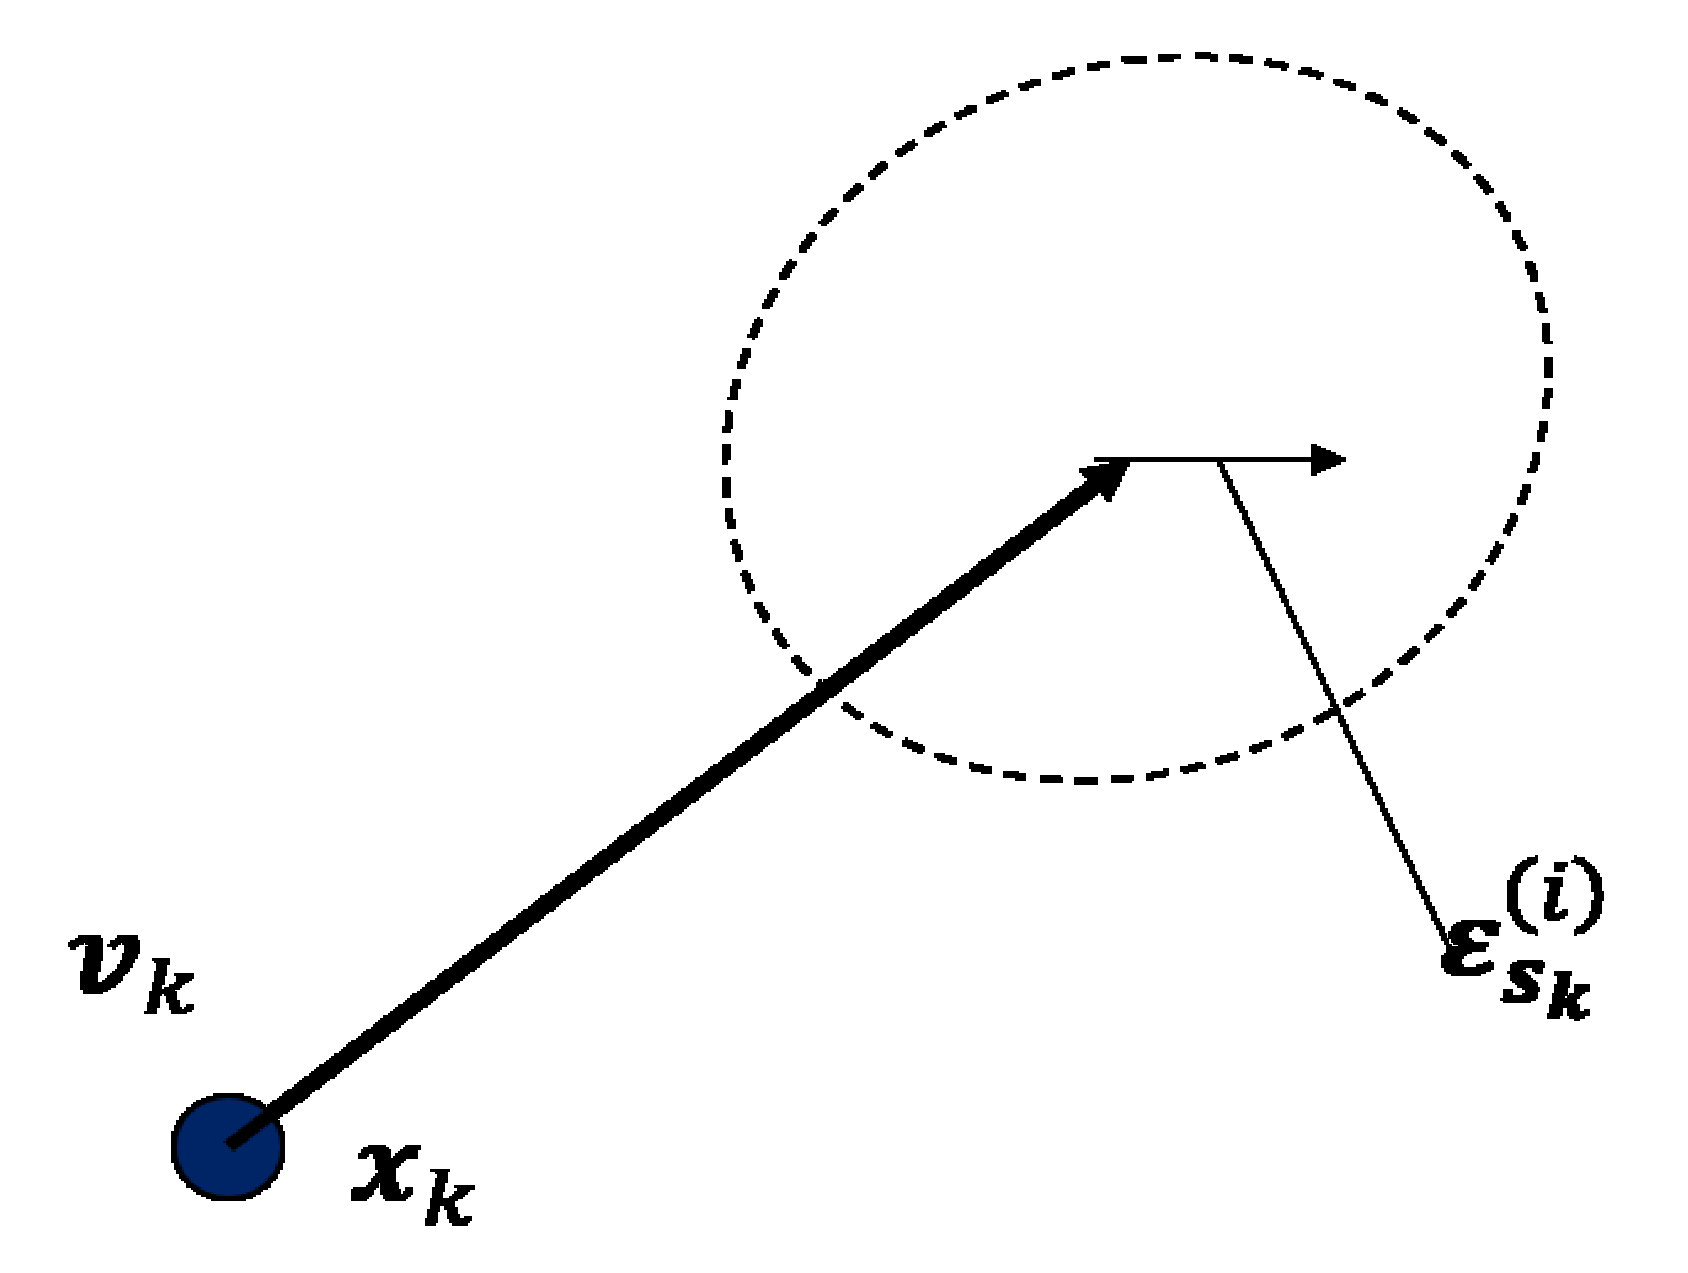
\includegraphics [height=5.0cm,width=5.0cm] {./fig/noise1.eps}
  \end{tabular}
 \end{center}
 \caption{$B%Q!<%F%#%/%k$N@8@.(B}\label{noise1}
\end{figure}


\newpage
 \item[Step 2:]{\bf $B=E$_(B($BL`EY(B)$B$N7W;;(B}\par
$BF;O)>pJs$H$7$F(B, ${\it{R}}=\{\vec{x} \mid
\vec{x}=\alpha(\vec{m}_{i+1}-\vec{m}_{i})+\vec{m}_{i}\}(0<\alpha\leq 1,
	       i=1,2,3,4)$$B$,$"$k$H$-(B,
	       $\hat{\vec{x}}_{k}^{(i)}=\vec{x}_{r}$$B$H$9$k$H(B, $\vec{m}_{i+1}-\vec{m}_{i}$
$B$H(B$\vec{x}_{r}-\vec{m}_{i}$$B$N3QEY(B$\theta$$B$O(B, 
$\cos \theta =\frac{(\vec{m}_{i+1}-\vec{m}_{i})\cdot
	       (\vec{x}_{r}-\vec{m}_{i})}{|\vec{m}_{i+1}-\vec{m}_{i}||\vec{x}_{r}-\vec{m}_{i}|}$
	        $(\vec{x}_{r}\neq
	       \vec{m}_{i})$
$B$h$j(B, $B5a$a$i$l$k(B. $B$7$?$,$C$F(B, $B%m%\%C%H$H$N5wN%(B$d_{k}$$B$O(B, 

\begin{equation}
  d_{k} = \left\{ \begin{array} {ll}
	  |\vec{x}_{r}-\vec{m}_{i}| & \textcircled{\scriptsize 1}(\cos{\theta}<0) \\
	  |\vec{x}_{r}-\vec{m}_{i}||\sin{\theta}| & \textcircled{\scriptsize 2}(0\leq
	  |\vec{x}_{r}-\vec{m}_{i}|cos{\theta}<|\vec{m}_{i+1}-\vec{m}_{i}|) \\
	  |\vec{x}_{r}-\vec{m}_{i+1}| & \textcircled{\scriptsize 3}(|\vec{x}_{r}-\vec{m}_{i}|cos{\theta}\geq |\vec{m}_{i+1}-\vec{m}_{i}|)
	  \end{array} \right.
\end{equation}

\begin{figure}[h]
 \begin{center}
  \begin{tabular}{cc}
   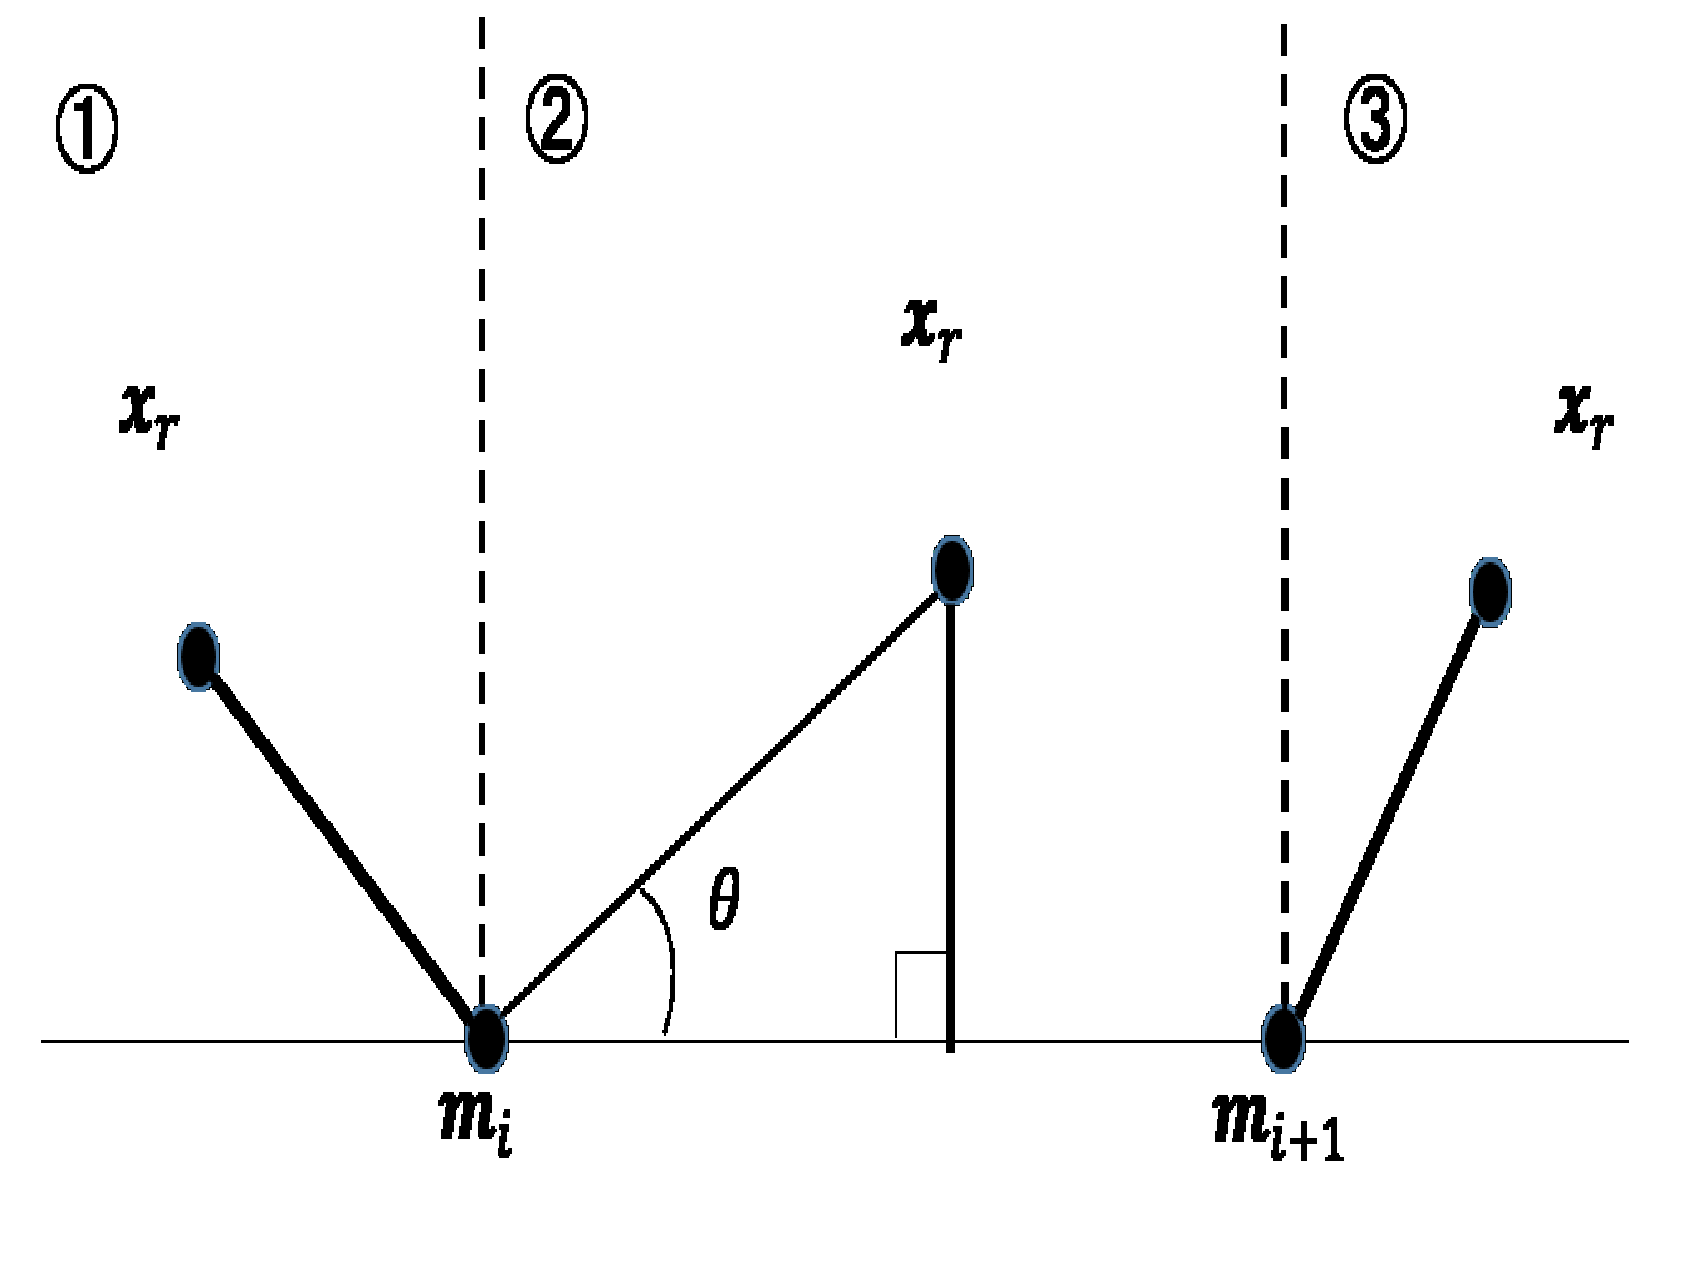
\includegraphics [height=5.0cm,width=10cm] {./fig/kyori.eps}
  \end{tabular}
 \end{center}
 \caption{$B%m%\%C%H$H$N5wN%(B}\label{kyori}
\end{figure}

$B$H5a$a$i$l$k(B. $B$3$l$rF;O)A4$F$G7W;;$7(B, 1$BHV>.$5$$$b$N$r:NMQ$9$k(B.
$B$3$l$h$j(B, $BCO?^>pJs$NL`EY$r(B
\begin{equation}
w_{1,k}^{[m]}=\left\{ \begin{array} {ll}
    1 & (d_{k}\leq W_{road}) \\
    (\exp(-\frac{(d_{k}-W_{road})^2}{A})+0.1)/1.1 & (d_{k}
	  > W_{road})
     \end{array} \right.
\end{equation}
$B$H5a$a$k(B. $B$?$@$7(B$A$$B$OD4@0$9$Y$-%Q%i%a!<%?(B, $W_{road}$$B$OF;I}$G$"$k!%(B
$B$^$?(B, $BJ}0L%;%s%5$N7WB,CM$r(B$\theta_k$$B$H$9$k!%J}0L%;%s%5$N7WB,CM$H?dDjCM$H$NL`EY$r(B
\begin{equation}
 w_{2,k}^{[m]}=\exp\left(-\frac{\theta_k^{[m]}-\theta_k)^2}{B}\right)
\end{equation}
$B$H5a$a$k!%$3$3$G!$(B$B$$B$OD4@0$9$Y$-%Q%i%a!<%?$G$"$k(B.
$B$3$l$i$NL`EY$r;H$$@55,2=A0$N%Q!<%F%#%/%k$NL`EY$r(B
\begin{equation}
w_{3,k}^{[m]}=Cw_{1,k}^{[m]}+(1-C)w_{2,k}^{[m]}
 \label{w:eq}
\end{equation}
$B$H$9$k!%$3$3$G!$(B$C$$B$OD4@0$9$Y$-%Q%i%a!<%?$G$"$k(B. $B<0(B(\ref{w:eq})$B$r@55,2=$9$k$3$H$G3F%Q!<%F%#%/%k$NL`EY$r<!$N$h$&$K5a$a$k!%(B
\begin{equation}
 w_{k}^{[m]}=\frac{w_{3,k}^{[m]}}{\sum_{m=1}^{M} w_{3,k}^{[m]}}
\end{equation}\\
\newpage
 \item[Step 3:]{\bf $B%j%5%s%W%j%s%0(B}\par
$B:G8e$KL`EY7W;;$K$h$C$F3F%Q!<%F%#%/%k$NJ,I[$,JP$C$F$7$^$C$?>l9g(B
$B%j%5%s%W%j%s%0$r9T$&!%K\8&5f$G$O%j%5%s%W%j%s%0$r9T$&>r7o$H$7$F(B
$B<!<0$K<($9M-8z%5%s%W%k%5%$%:(B(ESS:Effective~\\Sample~Size)$B$r(B
$BMxMQ$7$3$NCM$,%Q!<%F%#%/%k?t$NH>J,0J2<$K$J$C$?$H$-$N$_(B
$B%j%5%s%W%j%s%0$r9T$&!$(B
\begin{eqnarray}
 N_{\rm ess}=\left(\sum_m (w_k^{[m]})^2\right)^{-1} \label{ESS}
\end{eqnarray}
$B%j%5%s%W%j%s%0$O2>$N%Q!<%F%#%/%k=89g(B
$\bigl< \tilde{\vec{X}}_{k}^{[m]} \bigr>_{m=1}^M$
$B$NCf$N>uBVJQ?t$N3FMWAG(B$\tilde{\vec{x}}_k^{[m]}$$B$r3F%Q!<%F%#%/%k$N(B
$BL`EY(B$\tilde{w}_{k}^{[m]}$$B$KHfNc$7$?3NN($GI|85Cj=P$r9T$&!%(B
\begin{eqnarray}
 \vec{x}_{k}^{[m]} &\sim& \left\{
			   \begin{array}{c}
			    \tilde{\vec{x}}_k^{[1]}~\text{with~prob.}
			     \propto \tilde{w}_k^{[1]}\\
			    \tilde{\vec{x}}_k^{[2]}~\text{with~prob.}
			     \propto \tilde{w}_k^{[2]}\\
			    \vdots\\
			    \tilde{\vec{x}}_k^{[M]}~\text{with~prob.}
			     \propto \tilde{w}_k^{[M]}\\
			   \end{array}\right.\\
 w_{k}^{[m]} &:=& \frac{1}{M}
\end{eqnarray}
$\tilde{w}_{k}^{[m]}$$B$,Bg$-$$$[$ICj=P$5$l$k3NN($O9b$/$J$k$N$G!$(B
$B%j%5%s%W%j%s%08e$N=89g$K$O=EJ#$9$k%Q!<%F%#%/%k$,B?$/4^$^$l$F$$$k!%0J>e$N(B
$B<j=g$K$h$j;~9o(B$k$$B$N(BPF$B$NJ,I[$r6a;w$9$k%Q!<%F%#%/%k72$,F@$i$l$k!%(B
\begin{equation}
 \bigl< \vec{X}_{k}^{[m]} \bigr>_{m=1}^M
  =\bigl< \vec{x}_k^{[m]},w_k^{[m]} \bigr>_{m=1}^M
\end{equation}
$B0J>e$N(B$3$$B%9%F%C%W$N=hM}$r9T$&$3$H$K$h$j!$3F;~9o$K$*$1$kL\I8J,I[!$$9$J$o$A;~9o(B$k$
$B$G$N<+8J;Q@*$r<!<0$K$h$C$F?dDj$G$-$k!%(B
\begin{equation}
 \bar{\vec{x}}_k=\left(
		 \begin{array}{c}
		  \bar{x}_k\\
		  \bar{y}_k\\
		  \bar{z}_k\\
		  \bar{\theta}_k\\
		 \end{array}
		 \right)
 =\sum_{m=1}^M w_k^{[m]}\vec{x}_k^{[m]}
\end{equation}

\end{enumerate}

\newpage
\section{$B<B83(B}
 \subsection{$B;HMQ5!4o(B}
  $BK\8&5f$O!$0\F0%m%\%C%H$K(BMobileRobots$B<R$N(BP3-AT$B?^(B\ref{P3-AT}$B!$CO<'5$J}0L%;%s%5$K(BHoneywell$B<R$N(BHMC6352$B!$(BRGB-D$B%+%a%i(B
$B7s?<EY%;%s%5$K(BXbox One Kinect$B%;%s%5?^(B\ref{Kinect$B%;%s%5(B}$B$rMQ$$$k!%(BKinect
$B%;%s%5$N;EMM$K$D$$$FI=(B\ref{kinect$B%;%s%5$N;EMM(B}$B$K<($9(B.
%%kinect$B;EMM(B
\begin{table}[h]
  \begin{center}
   \caption{Kinect$B%;%s%5$N;EMM(B}\label{kinect$B%;%s%5$N;EMM(B}
   \begin{tabular}{|c|c|c|}
    \hline
    & $B2rA|EY(B & 1920$B!_(B1080 \\ \cline{2-3}
    $B?'(B& $B%U%l!<%`%l!<%H(B & 30[fps] \\ \cline{2-3}
    & $B%U%l!<%`%l!<%H(B($B0E=j(B) & 15[fps] \\ \hline
    & $BB,DjHO0O(B & 0.5 $\sim$ 8.0[m]\\ \cline{2-3}
    $B?<EY(B & $B2rA|EY(B & 512$B!_(B424 \\ \cline{2-3}
    & $B?<EY%U%l!<%`%l!<%H(B & 30[fps] \\ \hline
    $B?eJ?3QEY(B & \multicolumn{2}{|c|}{70[deg]} \\ \hline
    $B?bD>3QEY(B & \multicolumn{2}{|c|}{60[deg]} \\ \hline
    \end{tabular}
   \end{center}
\end{table}
%%P3-AT
\begin{figure}[h]
\begin{center}
\begin{tabular}{cc}
\includegraphics [width=9.0cm,angle=270] {./fig/rob.eps}
\end{tabular}
\end{center}
\caption{P3-AT}\label{P3-AT}
\end{figure}
%%Kinect
\begin{figure}[h]
\centering
\begin{tabular}{cc}
\includegraphics [width=9.0cm]{./fig/Kinect.eps}
\end{tabular}
\caption{Kinect$B%;%s%5(B}\label{Kinect$B%;%s%5(B}
\end{figure}
 \subsection{$B<B83J}K!(B}
  $B<B83$O6e=#9)6HBg3X650i8&5f(B3$B9fEo<~0O$r(BP3-AT$B$r%8%g%$%9%F%#%C%/$K$h$k<jF0A`:n$GAv(B
$B9T$5$;!$CO<'5$J}0L%;%s%5$H(BKinect$B%;%s%5$N%G!<%?$r<hF@$9$k(B. Kinect$B%;%s%5$+$iF@$i$l$k%G!<%?$h$j!$<+8J;Q@*(B
$B?dDj$r9T$&!%$^$?!$(BKinect$B%;%s%5$+$iF@$i$l$k3F;~9o$G$N<+8J0LCV$r(BPF$B$K$h$k<+8J;Q@*(B
$B?dDj$KMQ$$$k$?$a$K!$(BKinect$BD>8r:BI8$rKL$r(B$y$$B<4J}(B
$B8~!$El$r(B$x$$B<4J}8~$H$7$?!$@$3&:BI87O$X$HJQ49$9$k!%Av9T7PO)$r?^(B\ref{$BAv9T7PO)(B}$B$K(B
$B<($9(B. 

%%$B7PO)(B
\begin{figure}[h]
\centering
\begin{tabular}{cc}
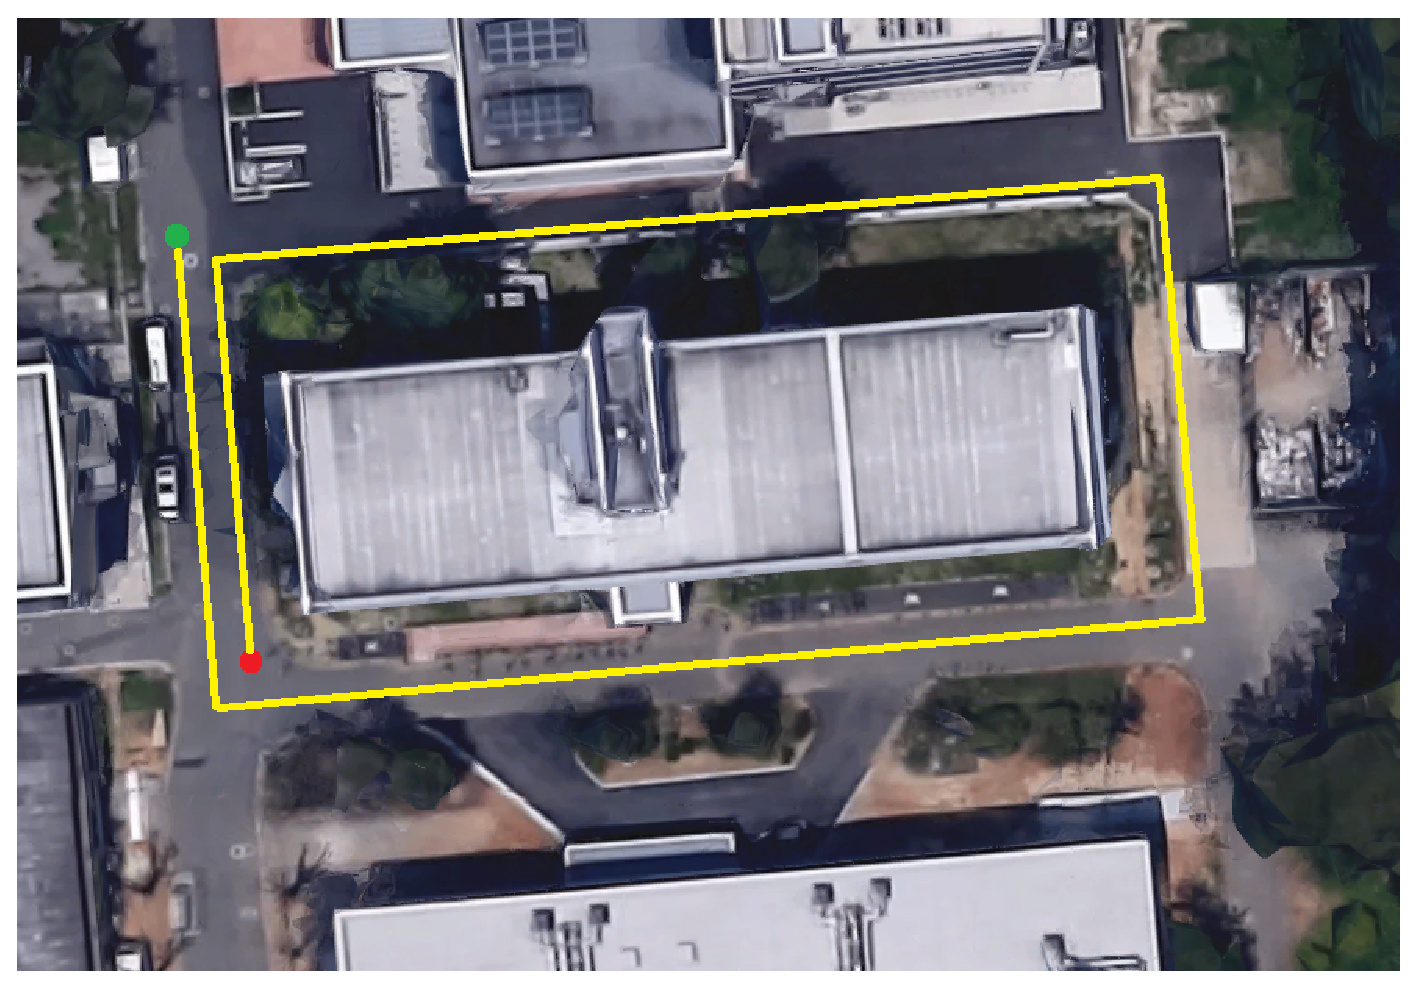
\includegraphics [width=9cm] {./fig/soukoukeiro2017.eps}
\end{tabular} 
\caption{$BAv9T7PO)(B}\label{$BAv9T7PO)(B}
\end{figure}

\begin{comment}
\newpage
GPS$B%G!<%?$OKL0^!$El7P!$1R@1JdB-?t$H$7$FF@$i$l$k!%(BGPS$B:BI8$r@$3&:BI8$X$HJQ49$9$k!%;~9o(B$k$$B$G$NKL0^!$El7P$r(B$\acute{N}_{k}$$B!$(B$\acute{E}_{k}$$B$H$9$k$H!$El7P$NJQ49$O(B
\begin{equation}
 \acute{x}_{k}
  =(\acute{E}_{k}-\acute{E}_{0})
  \frac{\beta}{360}\
  \cos\left(\frac{\pi\acute{N}_{0}}{180}\right)
\end{equation}
$B$H$J$k!%$3$3$G(B$\beta$$B$O@VF;D9$G(B$40075.017$[km]$B$G$"$k!%F1;~$KKL0^$O(B
\begin{equation}
 \acute{y}_{k}=(\acute{N}_{k}-\acute{N}_{0})\frac{\pi\gamma}{360}
\end{equation}
$B$H$J$k!%$3$3$G(B$\gamma$$B$OKL6K$HFn6K$r7k$s$@D>7B$G(B$12756.274$[km]$B$G$"$k!%(B
\par
\end{comment}


\newpage
 \subsection{$B<B837k2L$H9M;!(B}
$B!!(B\subsubsection{PF$B$K$h$k?dDj7k2L$H9M;!(B}
  $BAv9T<B838e(B, Kinect$B%;%s%5$K$h$jF@$i$l$?(B3$B<!85(BSLAM$B$H$=$N(B3$B<!85(BSLAM$B$N<+8J;Q@*?dDj(B
$B7k2L$r%Q!<%F%#%/%k%U%#%k%?$K$h$j=$@5$r9T$C$?7k2L$r?^(B\ref{3d}$B$K<($9(B. $B$3$l$h$j(B, $BL`(B
$BEY7W;;$KCO?^>pJs$,MQ$$$i$l$?$b$N$O(B, 3$B<!85(BSLAM$B$N<+8J;Q@*?dDj(B
$B7k2L$r=$@5$7(B, $BCO?^%G!<%?$K6a$$$H$3$m$r?d0\$7$F$$$k$3$H$,$o$+$k(B. $B$^$?(B, $BL`(B
$BEY7W;;$KCO<'5$J}0L%;%s%5$7$+MQ$$$i$l$F$$$J$$$b$N$O(B, $B$&$^$/(B3$B<!85(BSLAM$B$N<+8J;Q@*?dDj(B
$B7k2L$r=$@5$G$-$F$$$J$$$3$H$,$o$+$k(B.
$B?^(B\ref{3d}$B$r(B$xy$$BJ?LL$K<M1F$7(B, $B??$N7PO)$H$7$?CO?^>pJs(B
$B$NCM$H(B, $B<+8J;Q@*?dDj7k2L$r(BPF$B$K$h$j=$@5$7$?CM$H$N(B, $BJ?6Q8m:9$H:GBg8m:9$r<($9$HI=$N$h$&$K$J$C$?!%$3$l$h$j(B, $BCO?^>pJs$K4X$9$kL`EY$N78?t$rBg$-$/$7$?J}$,$h$j@:EY$N9b$$=$@57k(B
$B2L$,F@$i$l$k$3$H$,J,$+$k(B.

\clearpage

\begin{figure}[h]
 \begin{center}
  \begin{tabular}{c}
   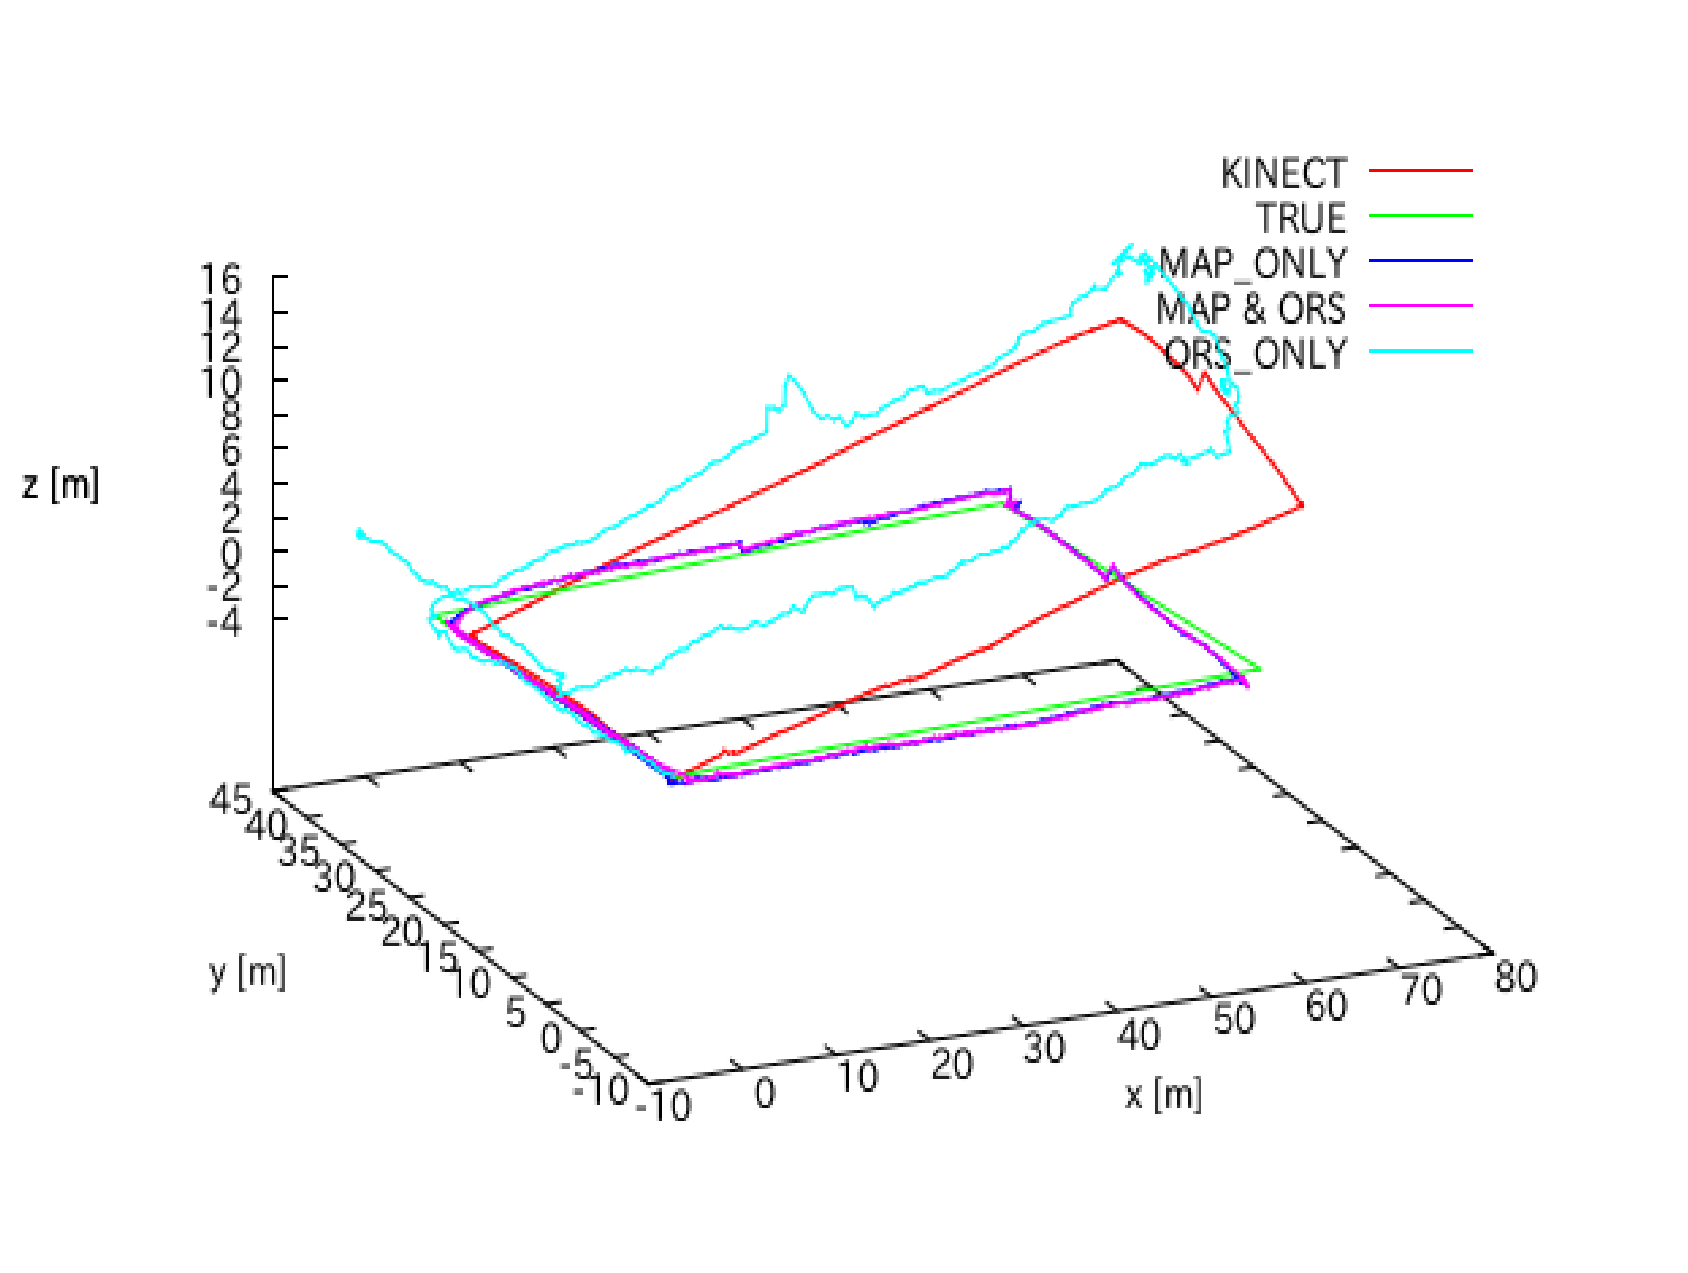
\includegraphics [height=8cm,width=11cm] {./fig/3dmap.eps}
   \end{tabular}
  \end{center}
 \caption{3$B<!85(BSLAM$B$N<+8J;Q@*?dDj7k2L$N=$@57k2L(B}\label{3d}
\end{figure}

\begin{figure}[h]
 \begin{center}
  \begin{tabular}{c}
   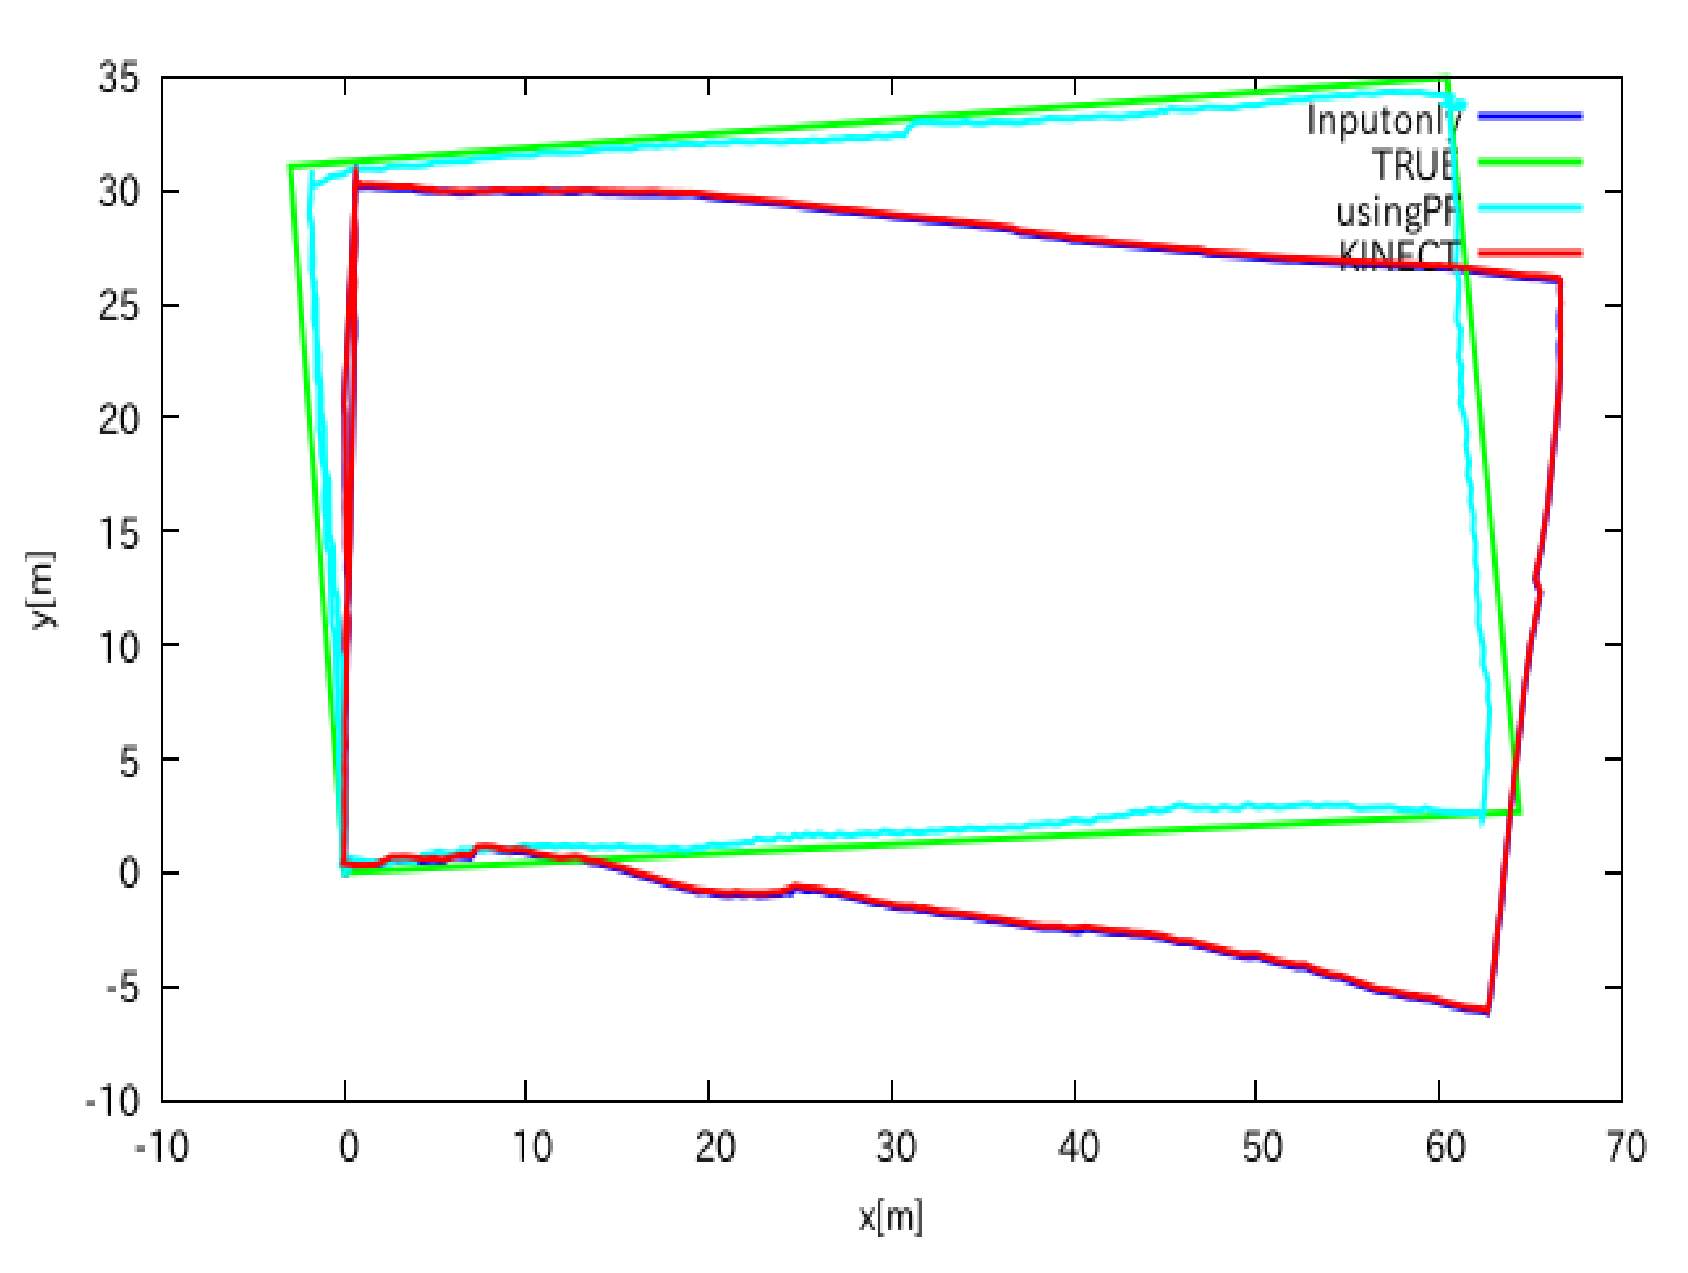
\includegraphics [height=8cm,width=11cm] {./fig/map_only.eps}
   \end{tabular}
  \end{center}
 \caption{(a)MAP\_ONLY($C$=1)}\label{map}
\end{figure}

\begin{figure}[h]
 \begin{center}
  \begin{tabular}{c}
   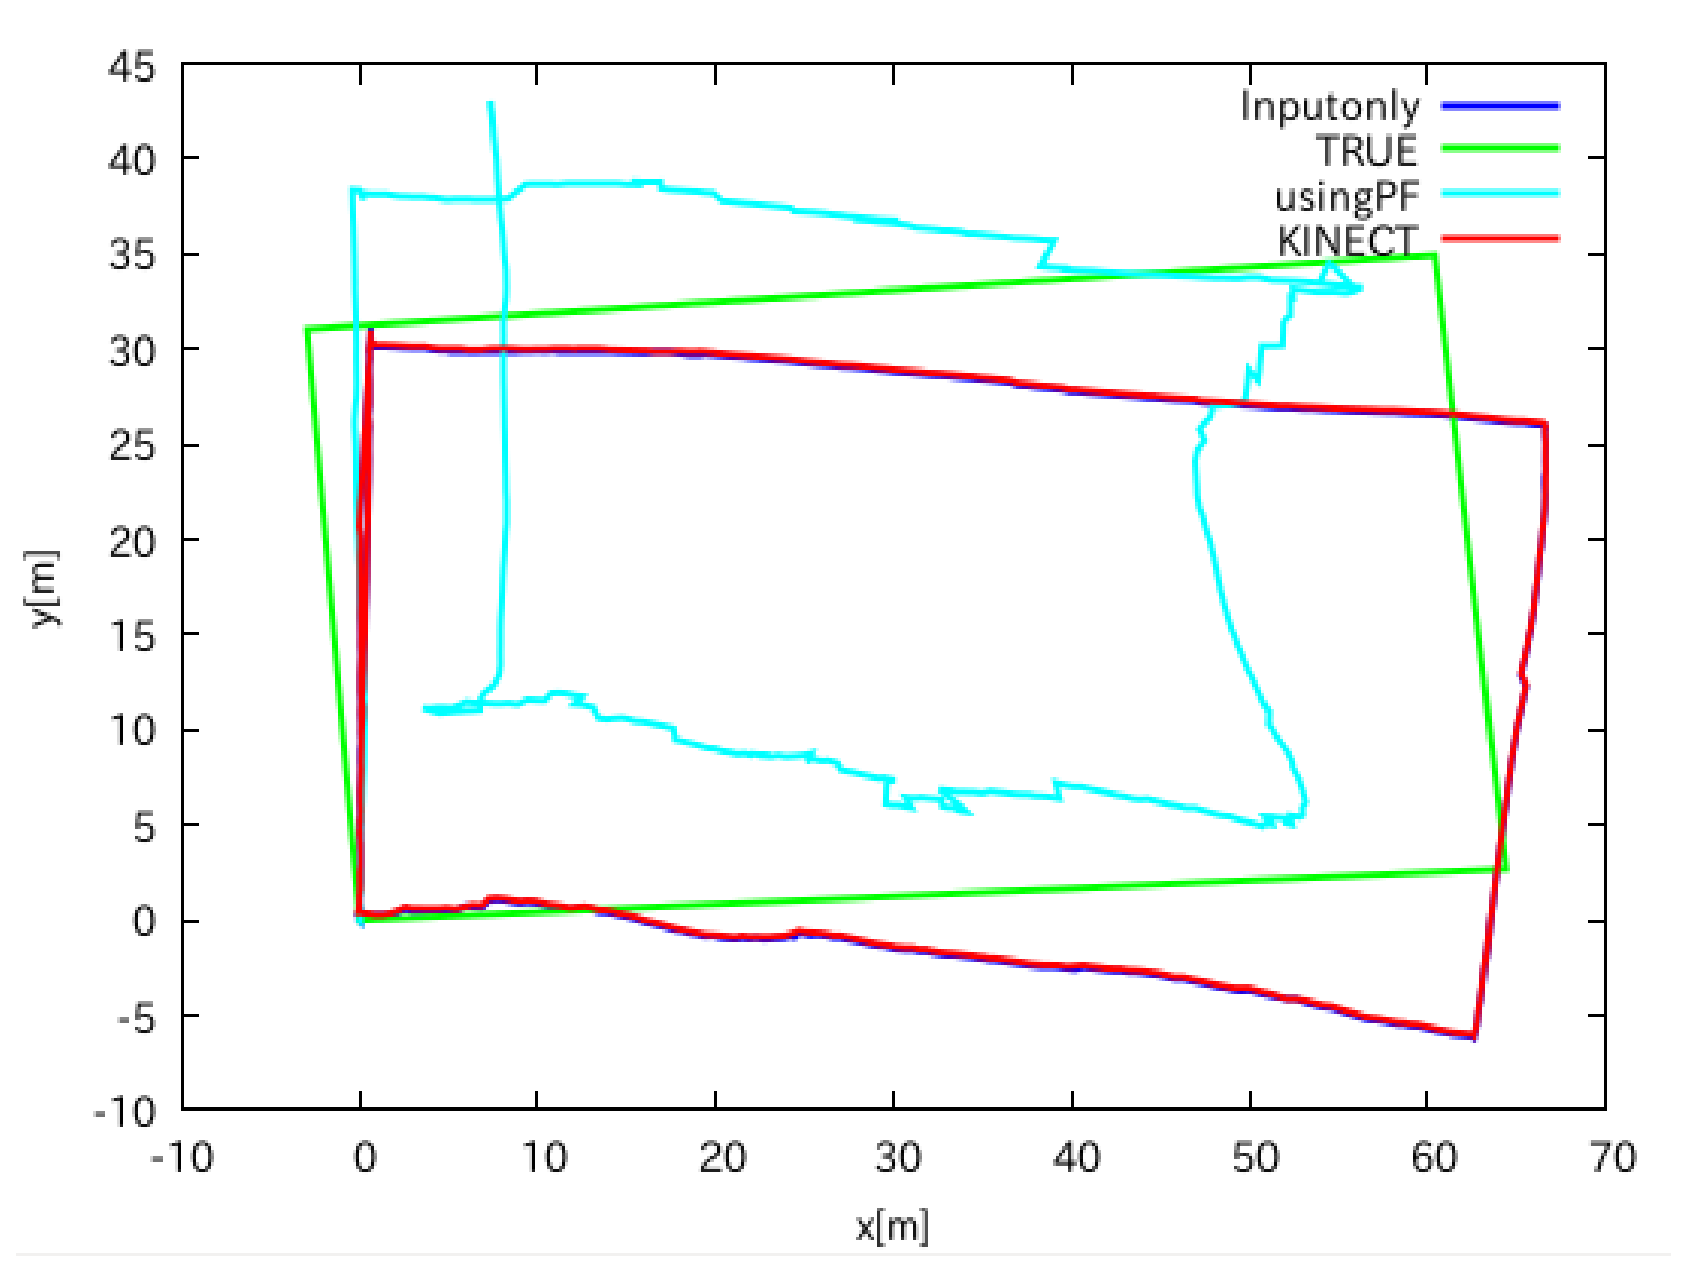
\includegraphics [height=8cm,width=11cm] {./fig/ors_only.eps}
   \end{tabular}
  \end{center}
 \caption{(b)ORS\_ONLY($C$=0)}\label{ors}
\end{figure}

\begin{figure}[h]
 \begin{center}
  \begin{tabular}{c}
   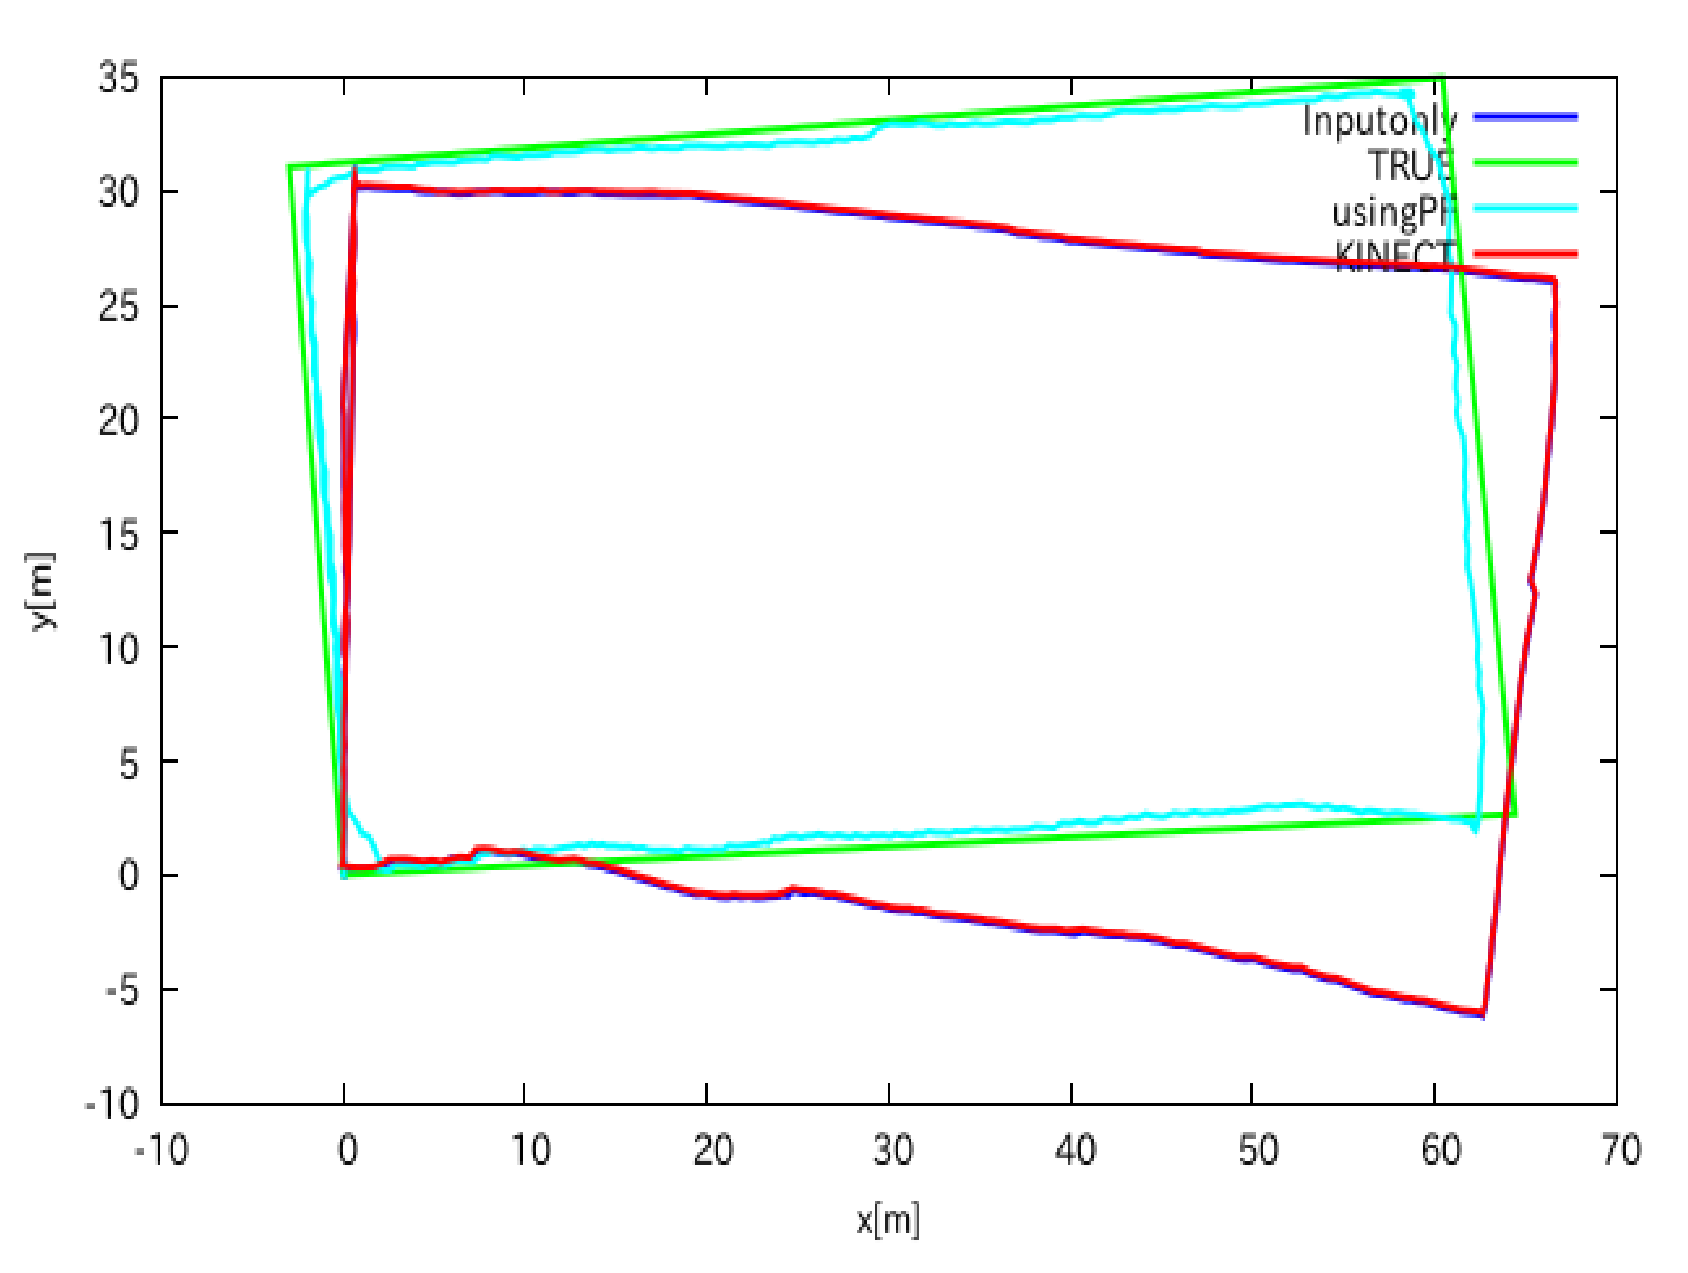
\includegraphics [height=8cm,width=11cm] {./fig/mapors.eps}
   \end{tabular}
  \end{center}
 \caption{(c)MAP\&ORS($C$=0.5)}\label{mapors}
\end{figure}




\begin{table}[h]
  \begin{center}
   \caption{$B??CM$H$N8m:9(B}
   \begin{tabular}{|c|c|c|}
    \hline
    & $BJ?6Q8m:9(B[m] & $B:GBg8m:9(B[m] \\ \hline
    (a)MAP\_ONLY & 0.527 & 1.51 \\ \hline
    (b)ORS\_ONLY & 5.28 & 14.2 \\ \hline
    (c)MAP\&ORS &  0.561 & 1.68 \\ \hline
    \end{tabular}
   \end{center}
\end{table}

\clearpage
\newpage
\section{$B7kO@(B}
  $BK\<B83$G(B, $BCO<'5$J}0L%;%s%5$HCO?^>pJs$rMQ$$$?%Q!<%F%#%/%k%U%#%k(B
$B%?$K$h$k(B3$B<!85<+8J;Q@*?dDj7k2L$r=$@5$9$kJ}K!$rDs0F$7(B, $B$=$N@:EY$rHf3S$7$?(B.
$B$=$N7k2L(B, $BL`EY7W;;$KCO?^>pJs$N$_$rMQ$$$?=$@57k2L$G$O(B, $BJ?6Q8m:9(B0.527[m],
$B:GBg8m:9(B1.51[m]$B$H@:EY$N9b$$=$@57k2L$,F@$i$l$?!%$^$?(B, $BCO<'5$J}0L%;%s%5$O(B,
3$B<!85<+8J;Q@*?dDj7k2L$N=$@5$K$"$^$jLrN)$?$J$$$3$H$,$o$+$C$?(B.
\par
$B:#8e$N2]Bj$H$7$F!$(BPF$B$KMQ$$$k$?$a$N(BGPS$B$NB,Dj8m:9$r8:>/$5$;$kJ}K!$N8!F$(B,
$B$^$?(B, $B<+8J;Q@*?dDj$K$*$1$k(B, $BCO<'5$J}0L%;%s%5$NM-MQ$JE,MQJ}K!$N8!F$$,$"$2$i$l$k!%(B


%%%% $B;29MJ88%(B %%%%
\newpage
\begin{thebibliography}{99}
 %\bibitem{name}name$B!$(B''paper name'',book name,page,year
 \bibitem{$BA0EDBsLm(B}$BA0EDBsLm!$(B''GPS$B$HCO<'5$J}0L%;%s%5(B, $BCO?^>pJs$rMQ$$$k%Q!<%F%#%/%k%U%#%k%?$K$h$k20300\F0%m%\%C%H$N<+8J;Q@*?dDj(B''$B6e=#9)6HBg3XB46HO@J8!$(B2017$B!%(B
 \bibitem{$B0lLZAV(B}$B0lLZAV!$(B''GPS$B$HCO<'5$J}0L%;%s%5$*$h$S(BKinect$B%;%s%5$rMQ$$$k%Q!<%F%#%/%k%U%#%k%?$K$h$k20300\F0%m%\%C%H$N$?$a$N%*%s%i%$%s(BSLAM''$B6e=#9)6HBg3XB46HO@J8!$(B2017$B!%(B
 \bibitem{Thrun}S.Thrun$BB>!$(B''$B3NN(%m%\%F%#%/%9(B''$B!$KhF|%3%_%e%K%1!<%7%g%s%:!$(B2004.
\end{thebibliography}


%%%%$B<U<-(B%%%%
\newpage
 \newpage
\begin{center}{\Large $B<U<-(B}\end{center}
  $B:#2s$3$NO@J8$N:n@.5Z$SK\8&5f$r?J$a$k$KEv$?$j!$B?Bg$J$k8f6(NO!$8f;XF3$r(B
$BBW$-$^$7$?9uLZ=(0l65<x!$>>Hx0lLp=u65!$@u@nOBI'5;=Q?&0w$K?<$/46<U$9$k$H$H$b$K8|$/8fNi?=(B
$B$7>e$2$^$9(B. \\
$B!!$^$?!$$$$m$$$m$H1~1g!$6(NO!$=u8@$r$7$F$/$l$?9uLZ8&5f<<9=@.0w0lF1$K$b=E$M(B
$B$F46<U$7$^$9!%(B
\newpage


%%%% $BIUO?!!(B%%%%
\newpage
\section{$BIUO?(B}
 {\Large A $B%m%\%C%H$NB.EYF0:n%b%G%k(B}\par
$BK\O@J8$GMQ$$$?%m%\%C%H$NB.EYF0:n%b%G%k$K$D$$$F4J7i$K=R$Y$k!%(B
$B;~9o(B$k$$B$K$*$1$k%m%\%C%H$N;Q@*$r(B$\vec{x}_k=(x_k,y_k,\theta_k)$$B!$(B
$BF~NO$r(B$\vec{u}_k=(v_k,\omega_k)^T$$B$H$9$k!%(B
$BF~NO(B$\vec{u}_k$$B$K%N%$%:$,4^$^$l$J$$>l9g!$%m%\%C%H$NB.EY$O(B
$(v_{k-1},\omega_{k-1})$$B$G0lDj$G$"$j!$%m%\%C%H$OH>7B(B$r_k-1=\left|\frac{v_{k-1}}{\omega_{k-1}}\right|$
$B$N1_8L>e$r0\F0$9$k!%$3$N$H$-1_8L$NCf?4:BI8(B$(x_c,y_c)$$B$,(B
\begin{equation}
 x_c=x_{k-1}-\frac{v_{k-1}}{\omega_{k-1}}\sin{\theta_{k-1}}
  ~,~~
 y_c=y_{k-1}+\frac{v_{k-1}}{\omega_{k-1}}\cos{\theta_{k-1}}
\end{equation}
$B$G$"$k$3$H$rMQ$$$k$H!$(B$\Delta t_{k-1}$$B8e$N;Q@*(B$\vec{x}_k$$B$O(B
$\omega_{k-1} \neq 0$$B$N$H$-(B
\begin{equation}
 \label{model_e}
 \vec{x}_k=\vec{x}_{k-1}+\left[
			 \begin{array}{c}
			  -\frac{v_{k-1}}{\omega_{k-1}}\sin{\theta_{k-1}}
			   +\frac{v_{k-1}}{\omega_{k-1}}
			    \sin{(\theta_{k-1}+\omega_{k-1} \Delta t_{k-1})}\\
			  \frac{v_{k-1}}{\omega_{k-1}}\cos{\theta_{k-1}}
			   -\frac{v_{k-1}}{\omega_{k-1}}
			    \cos{(\theta_{k-1}+\omega_{k-1} \Delta t_{k-1})}\\
			  \omega_{k-1} \Delta t_{k-1}\\
			\end{array}
			 \right]
\end{equation}
$B$H5a$a$i$l$k!%$J$*!$$3$N<0$O(B$\omega_{k-1}=0$$B$N$H$-$bK~$?$9!%(B
$BAvO)$N5/Iz$d<PLL$N$"$k20304D6-2<$G$O<B:]$NF~NO$O$3$N%b%G%k$K2C$(%N%$%:$,4^(B
$B$^$l$k>l9g$,$"$k!%$=$N$?$a%N%$%:$,2C$o$k>l9g$X$H3HD%$7$F9M$($k$?$a$K!$J?6Q$,%<%m$GM-8B$J(B
$BJ,;6$K=>$&3NN(JQ?t$G%b%G%k2=$r9T$&!%$7$?$,$C$F!$$3$N$H$-$N;~9o(B$k-1$$B$K$*$1(B
$B$k%m%\%C%H$N@)8fF~NO$O(B
$\vec{\hat{u}}_{k-1} = (\hat{v}_{k-1},\hat{\omega}_{k-1})^T
 = (v_{k-1},\omega_{k-1})^T
 + (\varepsilon_{\alpha_{1} v^2 + \alpha_{2} \omega^2}
 ,\varepsilon_{\alpha_{3} v^2 + \alpha_{4} \omega^2})^T$
$B$HI=$;$k!%$3$l$r<0(B(\ref{model_e})$B$KBeF~$7$?$b$N$rK\O@J8$G$NB.EYF0:n%b%G(B
$B%k$H$7$F07$&!%(B

\newpage
 {\Large B $B%Q!<%F%#%/%k%U%#%k%?$N?t3XE*F3=P(B}\par
$BN%;6;~9o(B$k=0,1,2,\cdots$$B$K$*$1$k>uBV(B$\vec{x}_{k}$$B!$F~NO(B$\vec{u}_{k}$$B!$(B
$B7WB,(B($B4QB,(B)$BCM(B$\vec{Z}_{k}$$B$KBP$7!$(B$\vec{x}_{k}$$B$O(BMarkov$B@-!$$9$J$o$A(B
$p(\vec{x}_{k}|\vec{x}_{0:k-1},\vec{u}_{1:k})=p(\vec{x}_{k}|\vec{x}_{k-1},\vec{u}_{k})$
$B$rK~$?$7!$$5$i$K$9$Y$F$N(B$k$$B$KBP$7!$4QB,Ns(B$\vec{Z}_{1},\cdots,\vec{Z}_{k}$$B$O(B
$B>uBVNs(B$\vec{x}_{0},\vec{x}_{1},\cdots,\vec{x}_{k}$$B$,4{CN$N>r7o2<$GFHN)(B
($B>r7oIUFHN)(B:~~CI:~conditionally~independent)$B$G$"$k$H2>Dj$9$k!%(B
$BNc$($P!$>uBV?d0\%b%G%k(B$p(\vec{x}_{k}|\vec{x}_{k-1},\vec{u}_{k})$$B$H(B
$B7WB,%b%G%k(B$p(\vec{Z}_{k}|\vec{x}_{k})$$B$,!$$=$l$>$l!$(B
\begin{eqnarray}
 \vec{x}_{k} &=& f(\vec{x}_{k-1},\vec{u}_{k})+\vec{\epsilon}_{k}
  \label{momodel:eq} \\
 \vec{Z}_{k} &=& g(\vec{x}_{k})+\vec{\delta}_{k}
  \label{mamodel:eq}
\end{eqnarray}
$B$GM?$($i$l$k@)8f7OEy$,9M$($i$l$k!%$3$3$G%7%9%F%`4X?t(B$f(\cdot)$$B$H(B
$B7WB,4X?t(B$g(\cdot)$$B$O7hDjO@E*(B(deterministic)$B$G$"$j!$%7%9%F%`8m:9(B
$\epsilon_{k}$$B$H7WB,8m:9(B$\delta_{k}$$B$O3NN(O@E*(B(stochastic)$B$G$"$k!%(B
$B<0(B(\ref{momodel:eq})$B$r>uBV?d0\%b%G%k(B($B%7%9%F%`%b%G%k!$F0:n%b%G%k!$1?F03X(B
$BE*%b%G%k(B)$B!$<0(B(\ref{mamodel:eq})$B$r7WB,%b%G%k$H$$$&!%(B\par
PF$B$GM=B,(B($B?dDj(B)$B$9$Y$->uBV$NNs(B$\vec{x}_{0},\vec{x}_{1},\cdots,\vec{x}_{k}$
$B$r(B$\vec{x}_{0:k}$$B$HI=$9$H!$$=$NF1;~3NN(J,I[$O0J2<$N$h$&$K$J$k!%(B
$B$^$:!$>r7oIU3NN($NDj5A<0$KA08~$-M=B,$N$_$K$h$j>uBV?dDj$9$k$H2>Dj$9$k$3$H(B
$B$K$h$j!$(B$p(\vec{x}_{k}|\vec{x}_{0:k-1},\vec{u}_{1:k},\vec{Z}_{1:k})$
$B$K$D$$$F$NA22=<0(B($B:F5"<0(B)
\begin{eqnarray}
 p(\vec{x}_{0:k}|\vec{u}_{1:k},\vec{Z}_{1:k})=p(\vec{x}_{k}|\vec{x}_{0:k-1},\vec{u}_{1:k},\vec{Z}_{1:k})p(\vec{x}_{0:k-1}|\vec{u}_{1:k-1},\vec{Z}_{1:k-1})
  \label{RP:eq}
\end{eqnarray}
$B$rF@$k!%$5$i$K!$$3$N<0$N1&JU$NBh(B1$B0x;R$N(B$\vec{x}_{k}$$B$NJ,I[$O!$$^$:(BMarkov
$B@-$K$h$j(B$\vec{x}_{k}$$B$NJ,I[$rM=B,(B($B?dDj(B)$B$7!$(BBayes$B$NDjM}$h$j7WB,CM(B
$\vec{Z}_{k}$$B$rMQ$$$F99?7(B($B=$@5(B)$B$7$F5a$a$k$3$H$H$9$k$H!$(B
\begin{eqnarray}
 p(\vec{x}_{k}|\vec{x}_{0:k-1},\vec{u}_{1:k},\vec{Z}_{1:k})
  &=&
  \frac{p(\vec{Z}_{k}|\vec{x}_{k},\vec{x}_{0:k-1},\vec{u}_{1:k},\vec{Z}_{1:k-1})p(\vec{x}_{k}|\vec{x}_{0:k-1},\vec{u}_{1:k},\vec{Z}_{1:k-1})}
  {p(\vec{Z}_{k}|\vec{x}_{0:k-1},\vec{u}_{1:k},\vec{Z}_{1:k-1})}\nonumber\\
 &=&
  \eta\hspace{0.5mm}p(\vec{Z}_{k}|\vec{x}_{k})p(\vec{x}_{k}|\vec{x}_{k-1},\vec{u}_{k})
  \label{BM:eq}
\end{eqnarray}
$B$,F@$i$l$k!%<0(B(\ref{BM:eq})$B$r<0(B(\ref{RP:eq})$B$KBeF~$7!$(B
$p(\vec{x}_{0:k}|\vec{u}_{1:k},\vec{Z}_{1:k})$
$B$r(B$r(\vec{x}_{k})$$B$H$*$$$FA22=<0(B
\begin{eqnarray}
 r(\vec{x}_{k}):=\eta\hspace{0.5mm}
  p(\vec{Z}_{k}|\vec{x}_{k})p(\vec{x}_{k}|\vec{x}_{k-1},\vec{u}_k)r(\vec{x}_{k-1})
  \label{TD:eq}
\end{eqnarray}
$B$,F@$i$l$k!%$3$N<0$+$i;~9o(B$k=1,2,\cdots$$B$KBP$7$F=g<!F@$i$l$k(B
$r(\vec{x}_{k})$$B$r;~9o(B$k$$B$K$*$1$k(BPF$B$NL\I8J,I[(B(target~distribution)
$B$H$9$k!%(B\par
PF$B$O!$A0;~9o$GF@$i$l$?L\I8J,I[(B($B$^$?$O$=$N6a;w(B)$B$+$i!$$"$kDs0FJ,I[(B
(proposal~distribution)$q(\vec{x}_{k})$$B$rN3;R(B(particle)$B$N=89g$H$7$FM=B,(B
$B@8@.$7!$=E$_(B$w_{k}$$B$K$h$j=$@5$7$?(B$w_{k}q(\vec{x}_{k})$$B$K$h$j3F;~9o$N(BPF$B$N(B
$BL\I8J,I[(B$p(\vec{x}_{0:k}|\vec{u}_{1:k},\vec{Z}_{1:k})$$B$r?dDj$9$k!%$^$?(B
$BL@$i$+$K(B
\begin{eqnarray}
 w_{k}=\frac{p(\vec{x}_{0:k}|\vec{u}_{1:k},\vec{Z}_{1:k})}{q(\vec{x}_{k})}
  =\frac{\rm $BL\I8J,I[(B}{\rm $BDs0FJ,I[(B}
\end{eqnarray}
$B$H$9$l$P$h$$$3$H$,$o$+$k!%:G$bD>@\E*$JJ}K!$O!$>uBV?d0\%b%G%k(B
$p(\vec{x}_{k}|\vec{x}_{k-1},\vec{u}_{k})$$B$rMQ$$$FDs0FJ,I[$r@8@.$7!$7WB,(B
$B%b%G%k(B$p(\vec{Z}_{k}|\vec{x}_{k})$$B$rMQ$$$?=E$_$G=$@5$9$k!%$9$J$o$A(B
\begin{eqnarray}
 q(\vec{x}_{k}) &:=&
  p(\vec{x}_{k}|\vec{x}_{k-1},\vec{u}_{k})q(\vec{x}_{k-1})\\
 w_{k} &:=&
  \eta\hspace{0.5mm}p(\vec{Z}_{k}|\vec{x}_{k})w_{k-1}
  \label{wt1:eq}
\end{eqnarray}
$B$H$7$F!$=i4|>r7o$r(B$q(\vec{x}_{0})=p(\vec{x}_{0})$$B$H(B$w_{0}=1/M$$B$H$7$F(B
$k=,1,2,\cdots$$B$K$D$$$F!$(B$w_{k}q(\vec{x}_{k})$$B$K$h$jL\I8J,I[$r?dDj$9$k(B
$B>l9g!$(B
$w_{k}q(\vec{x}_{k})=p(\vec{Z}_{k}|\vec{x}_{k})p(\vec{x}_{k}|\vec{x}_{k-1},\vec{u}_{k})\left[w_{k-1}q(\vec{x}_{k-1})\right]$
$B$H$J$k$N$G!$(B$w_{k}q(\vec{x}_{k})$$B$r@55,2=$9$l$P!$<0(B(\ref{TD:eq})$B$NL\I8J,(B
$BI[$HEy2A$K$J$k!%$J$*!$>e5-$N=E$_$O(BBayes$B$NDjM}$NL`EY(B
(likelihood)$p(\vec{Z}_{k}|\vec{x}_{k})$$B$KAjEv$9$k$N$G!$$=$&8F$V>l9g$b$"(B
$B$k!%(B\par
$B$5$i$K!$>e<0$N(B$q(\vec{x}_{k})$$B$H(B$w_{k}$$B$rCf4V$NJ,I[(B
$\tilde{q}(\vec{x}_{k})$$B$H=E$_(B$\tilde{w}_{k}$$B$H$7!$(B
$\tilde{q}(\vec{x}_{k})$$B$+$i=E$_(B$\tilde{w}_{k}$$B$G%j%5%s%W%j%s%0$7$FF@$?(B
$q(\vec{x}_{k}) \sim \tilde{w}_{k} \tilde{q}(\vec{x}_{k})$$B$rDs0FJ,I[!$?7(B
$B$7$$=E$_$r(B$w_{k}=1/M$$B$H$9$k$H!$(B$\sum w_{k}q(\vec{x}_{k})$$B$GL\I8J,I[$,?d(B
$BDj$G$-$k!%$?$@$7!$=E$_(B$w_{k}$$B$NJ,I[$NJP$j$,>.$5$$$N$K%j%5%s%W%j%s%0$r9T(B
$B$&$H!$%b%s%F%+%k%m8m:9$,L5MQ$K:.F~$9$k$3$H$K$J$j!$$+$($C$F?dDj$N@:EY$,0-(B
$B$/$J$k$N$G!$%j%5%s%W%j%s%0$O=E$_(B$w_{k}$$B$NJ,I[$NJP$j$,Bg$-$$>l9g$N$_$K9T(B
$B$($P$h$$!%
\end{document}
